\section{Écrans produits}
Plusieurs écrans exploitables ont été réalisés avec la nouvelle machine et l'ancienne machine pour les expositions suivantes au spray :
\begin{itemize}
    \item 5 secondes (ancienne machine + mesure manuelles)
    \item 10 secondes (ancienne machine + mesure manuelles)
    \item 15 secondes (nouvelle machine + mesure auto)
    \item 30 secondes (nouvelle machine + mesure auto)
    \item 60 secondes (nouvelle machine + mesure auto)
\end{itemize}
Par exploitables on entend qu'ils ressemblent visuellement au résultat attendu décrit dans la \autoref{sec:fab_ecran_sit_init}.
\begin{figure}[H]
    \centering
    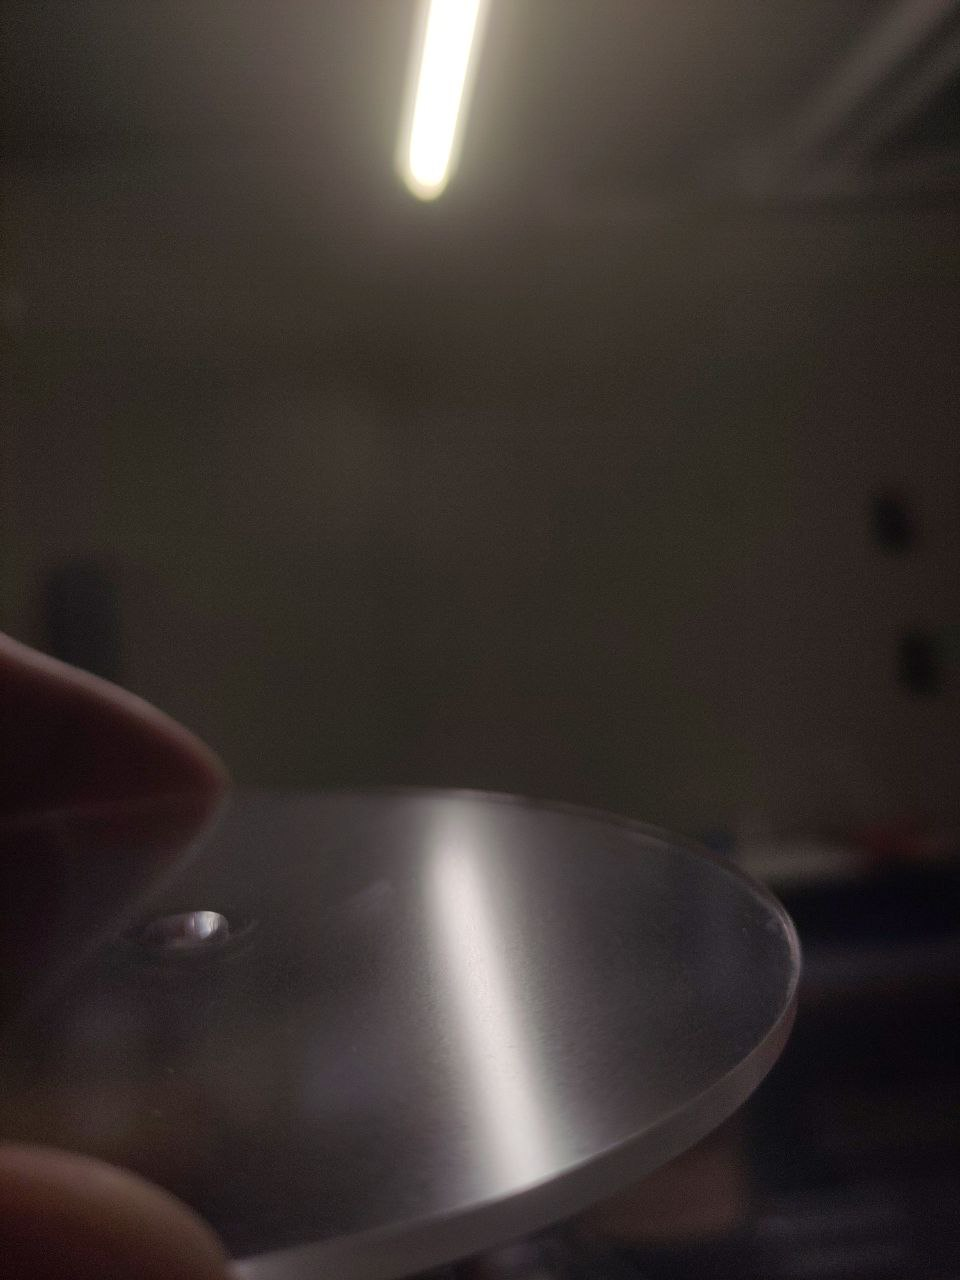
\includegraphics[width = 0.5\textwidth]{assets/figures/mesures/15_sec.jpeg}
    \caption{Écran 15 secondes}
\end{figure}

\begin{figure}[H]
    \centering
    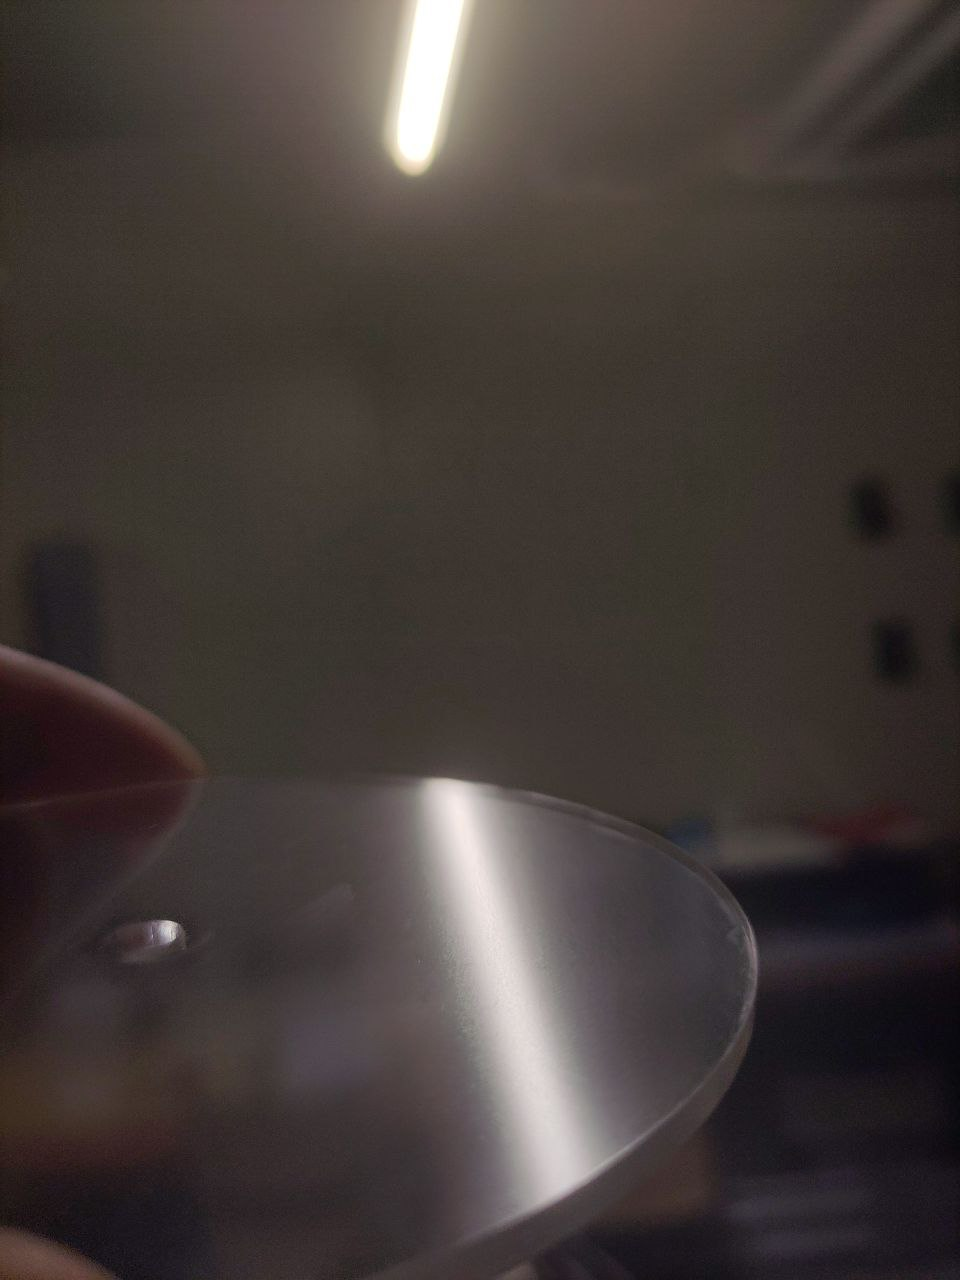
\includegraphics[width = 0.5\textwidth]{assets/figures/mesures/30_sec.jpeg}
    \caption{Écran 30 secondes}
\end{figure}

\begin{figure}[H]
    \centering
    \begin{subfigure}{.5\textwidth}
        \centering
        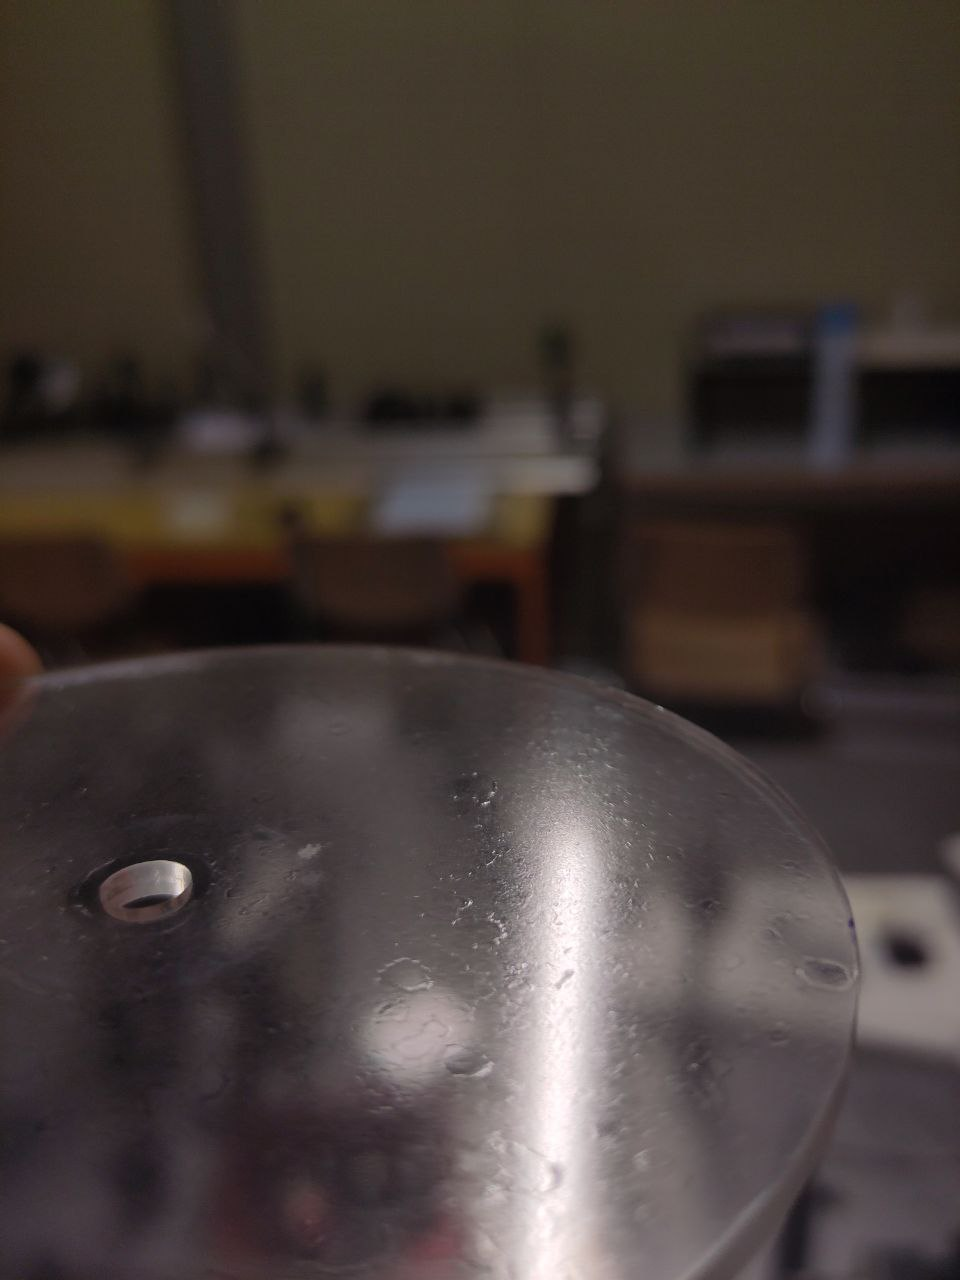
\includegraphics[width=1\linewidth]{assets/figures/mesures/60_sec.jpeg}
        \caption{Écran 60 secondes}
    \end{subfigure}%
    \begin{subfigure}{.5\textwidth}
        \centering
        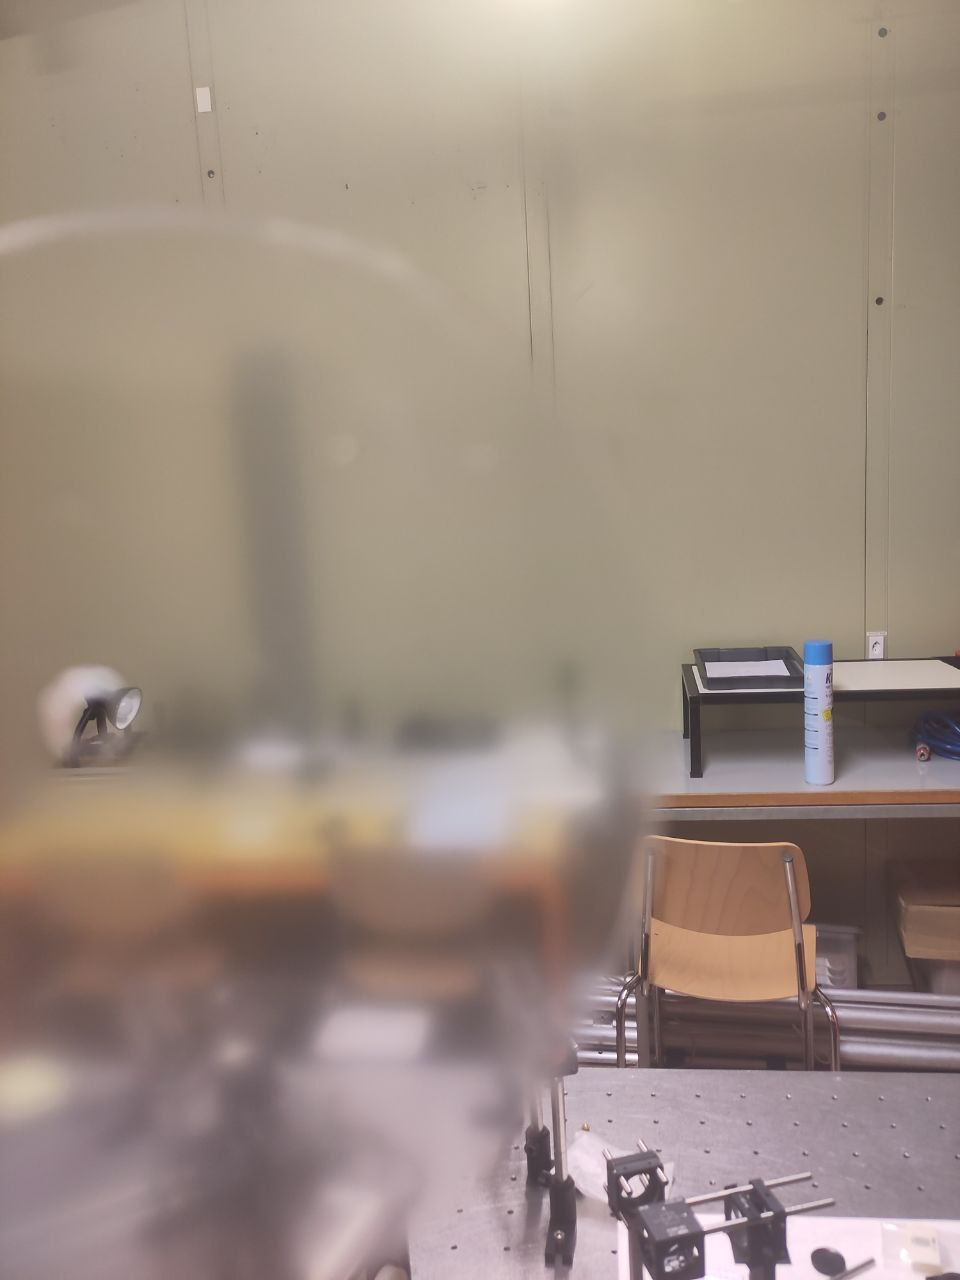
\includegraphics[width=1\linewidth]{assets/figures/mesures/60_sec_travers.jpeg}
        \caption{Vue au travers de l'écran de 60 secondes}
    \end{subfigure}
    \caption{Écran 60 secondes de côté et au-travers}
\end{figure}
Sur l'écran on peut observer des défaut, il y a eut des problèmes de buse lors de cette projection, il sera toutefois
intéressant de caractériser cet écran. Le nombre de prise de mesure est à chaque fois de 100 mesures.

\section{Script d'analyse des données}
Le script d'analyse des données est dans un état assez brut, en effet pour analyser des données, il faudra rentrer manuellement
le chemin du répertoire des fichiers de données :
\begin{figure}[H]
    \centering
    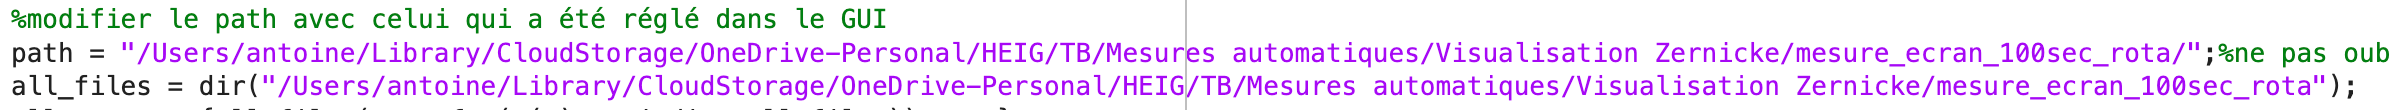
\includegraphics[width = 1\textwidth]{assets/figures/mesures/exemple_chemin_fichier.png}
    \caption{Exemple de chemin de fichier}
\end{figure}
Il faut alors modifier les lignes en rose, avec les chemin des dossier contenant les .csv des mesures.

En suite il suffit de lancer l'exécution du script, ce dernier soustrait automatiquement les mesures de références
faites sans écrans à toutes les mesures des coefficients de Zernike, il calculera la variance de toutes les séries de mesures :
\begin{equation}
    var = \frac{1}{N-1}\sum_{j=1}^{N}|a_j - \mu|
\end{equation}
Où $\mu$ est la moyenne des coefficients de Zernike $a_j$
\begin{equation}
    \mu = \frac{1}{N}\sum_{j=1}^{N}a_j
\end{equation}
Dans le code cela donne :
\begin{figure}[H]
    \centering
    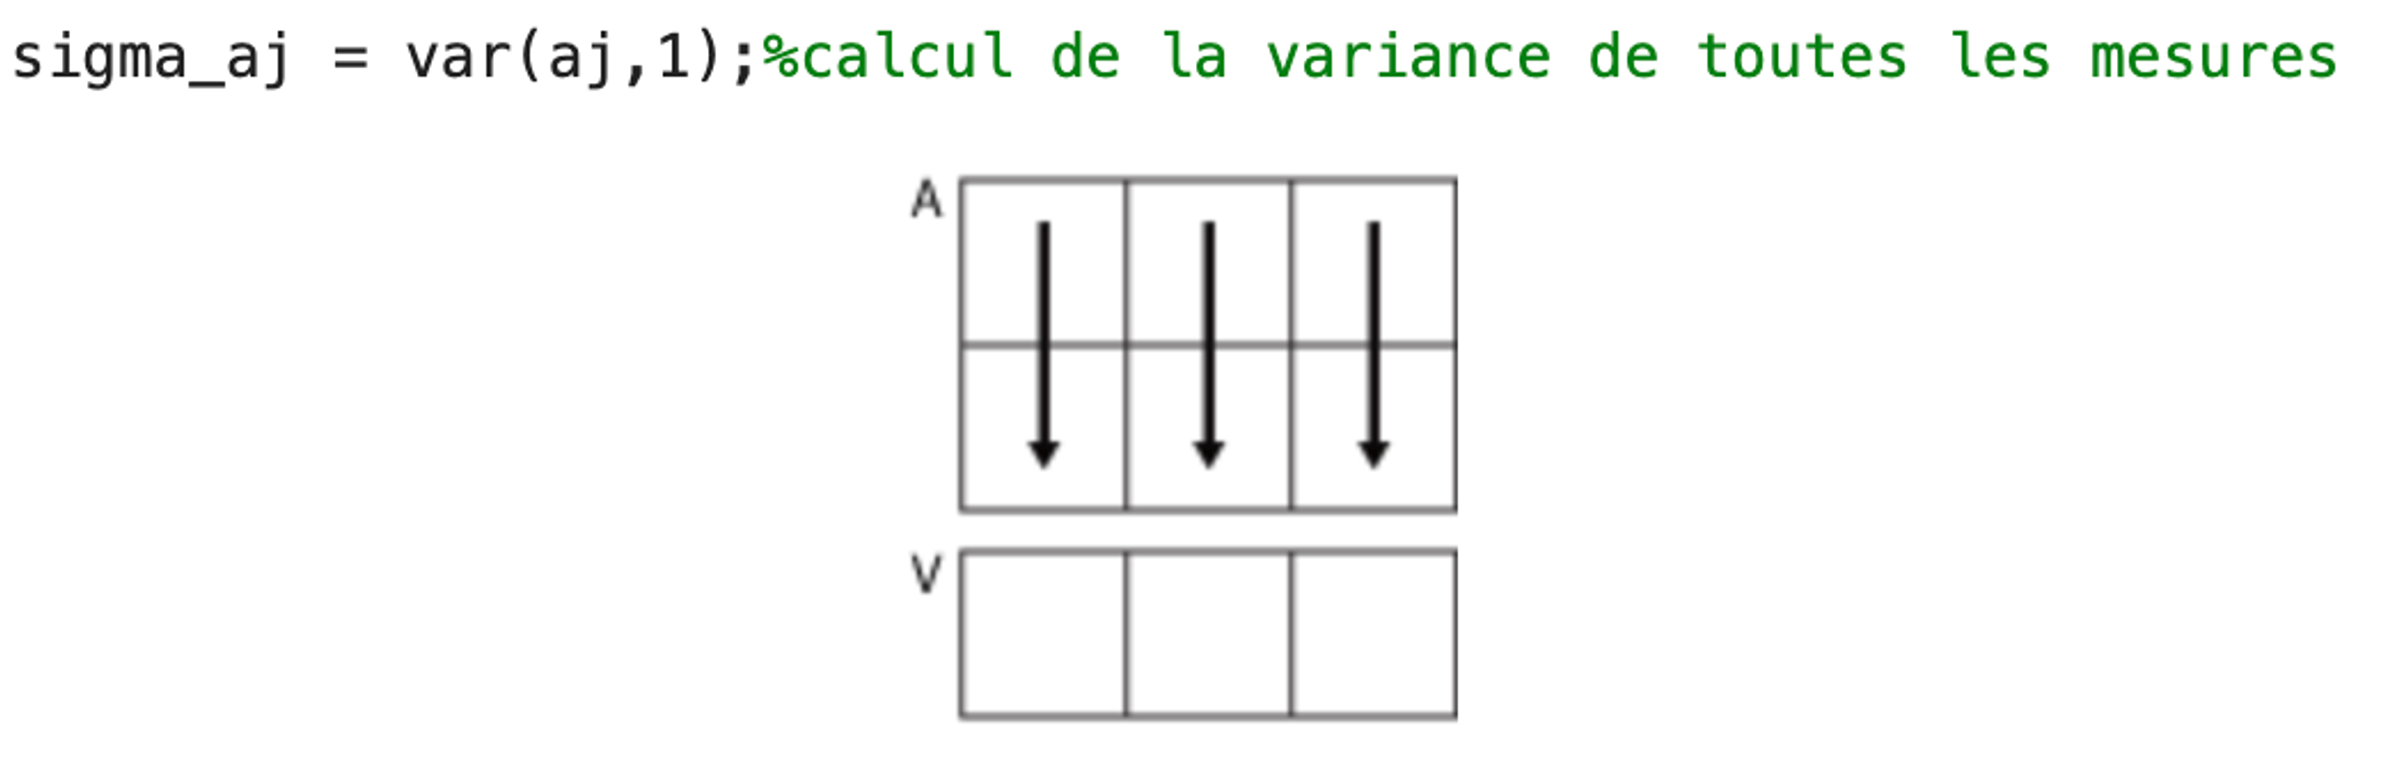
\includegraphics[width = 1\textwidth]{assets/figures/mesures/variance_matlab.png}
    \caption{Calcul de la variance des coefficients de Zernike}
\end{figure}
à la suite de ceci on obtient donc un tableau de dimension [1,66].

\newpage
En suite on utilise le fichier \textit{varianceNoll.m}, pour calculer les variances des coefficients de Zernike
pour $D/r_0 = 1$ :
\begin{figure}[H]
    \centering
    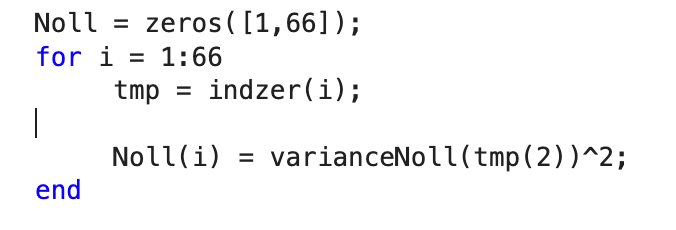
\includegraphics[width = 0.7\textwidth]{assets/figures/mesures/Calcul_variance_nool.png}
    \caption{Calcul des variances de Noll}
\end{figure}
En plottant les variances de Noll en fonction de leur indice j, à une échelle logarithmique, la courbe suivante est obtenue :
\begin{figure}[H]
    \centering
    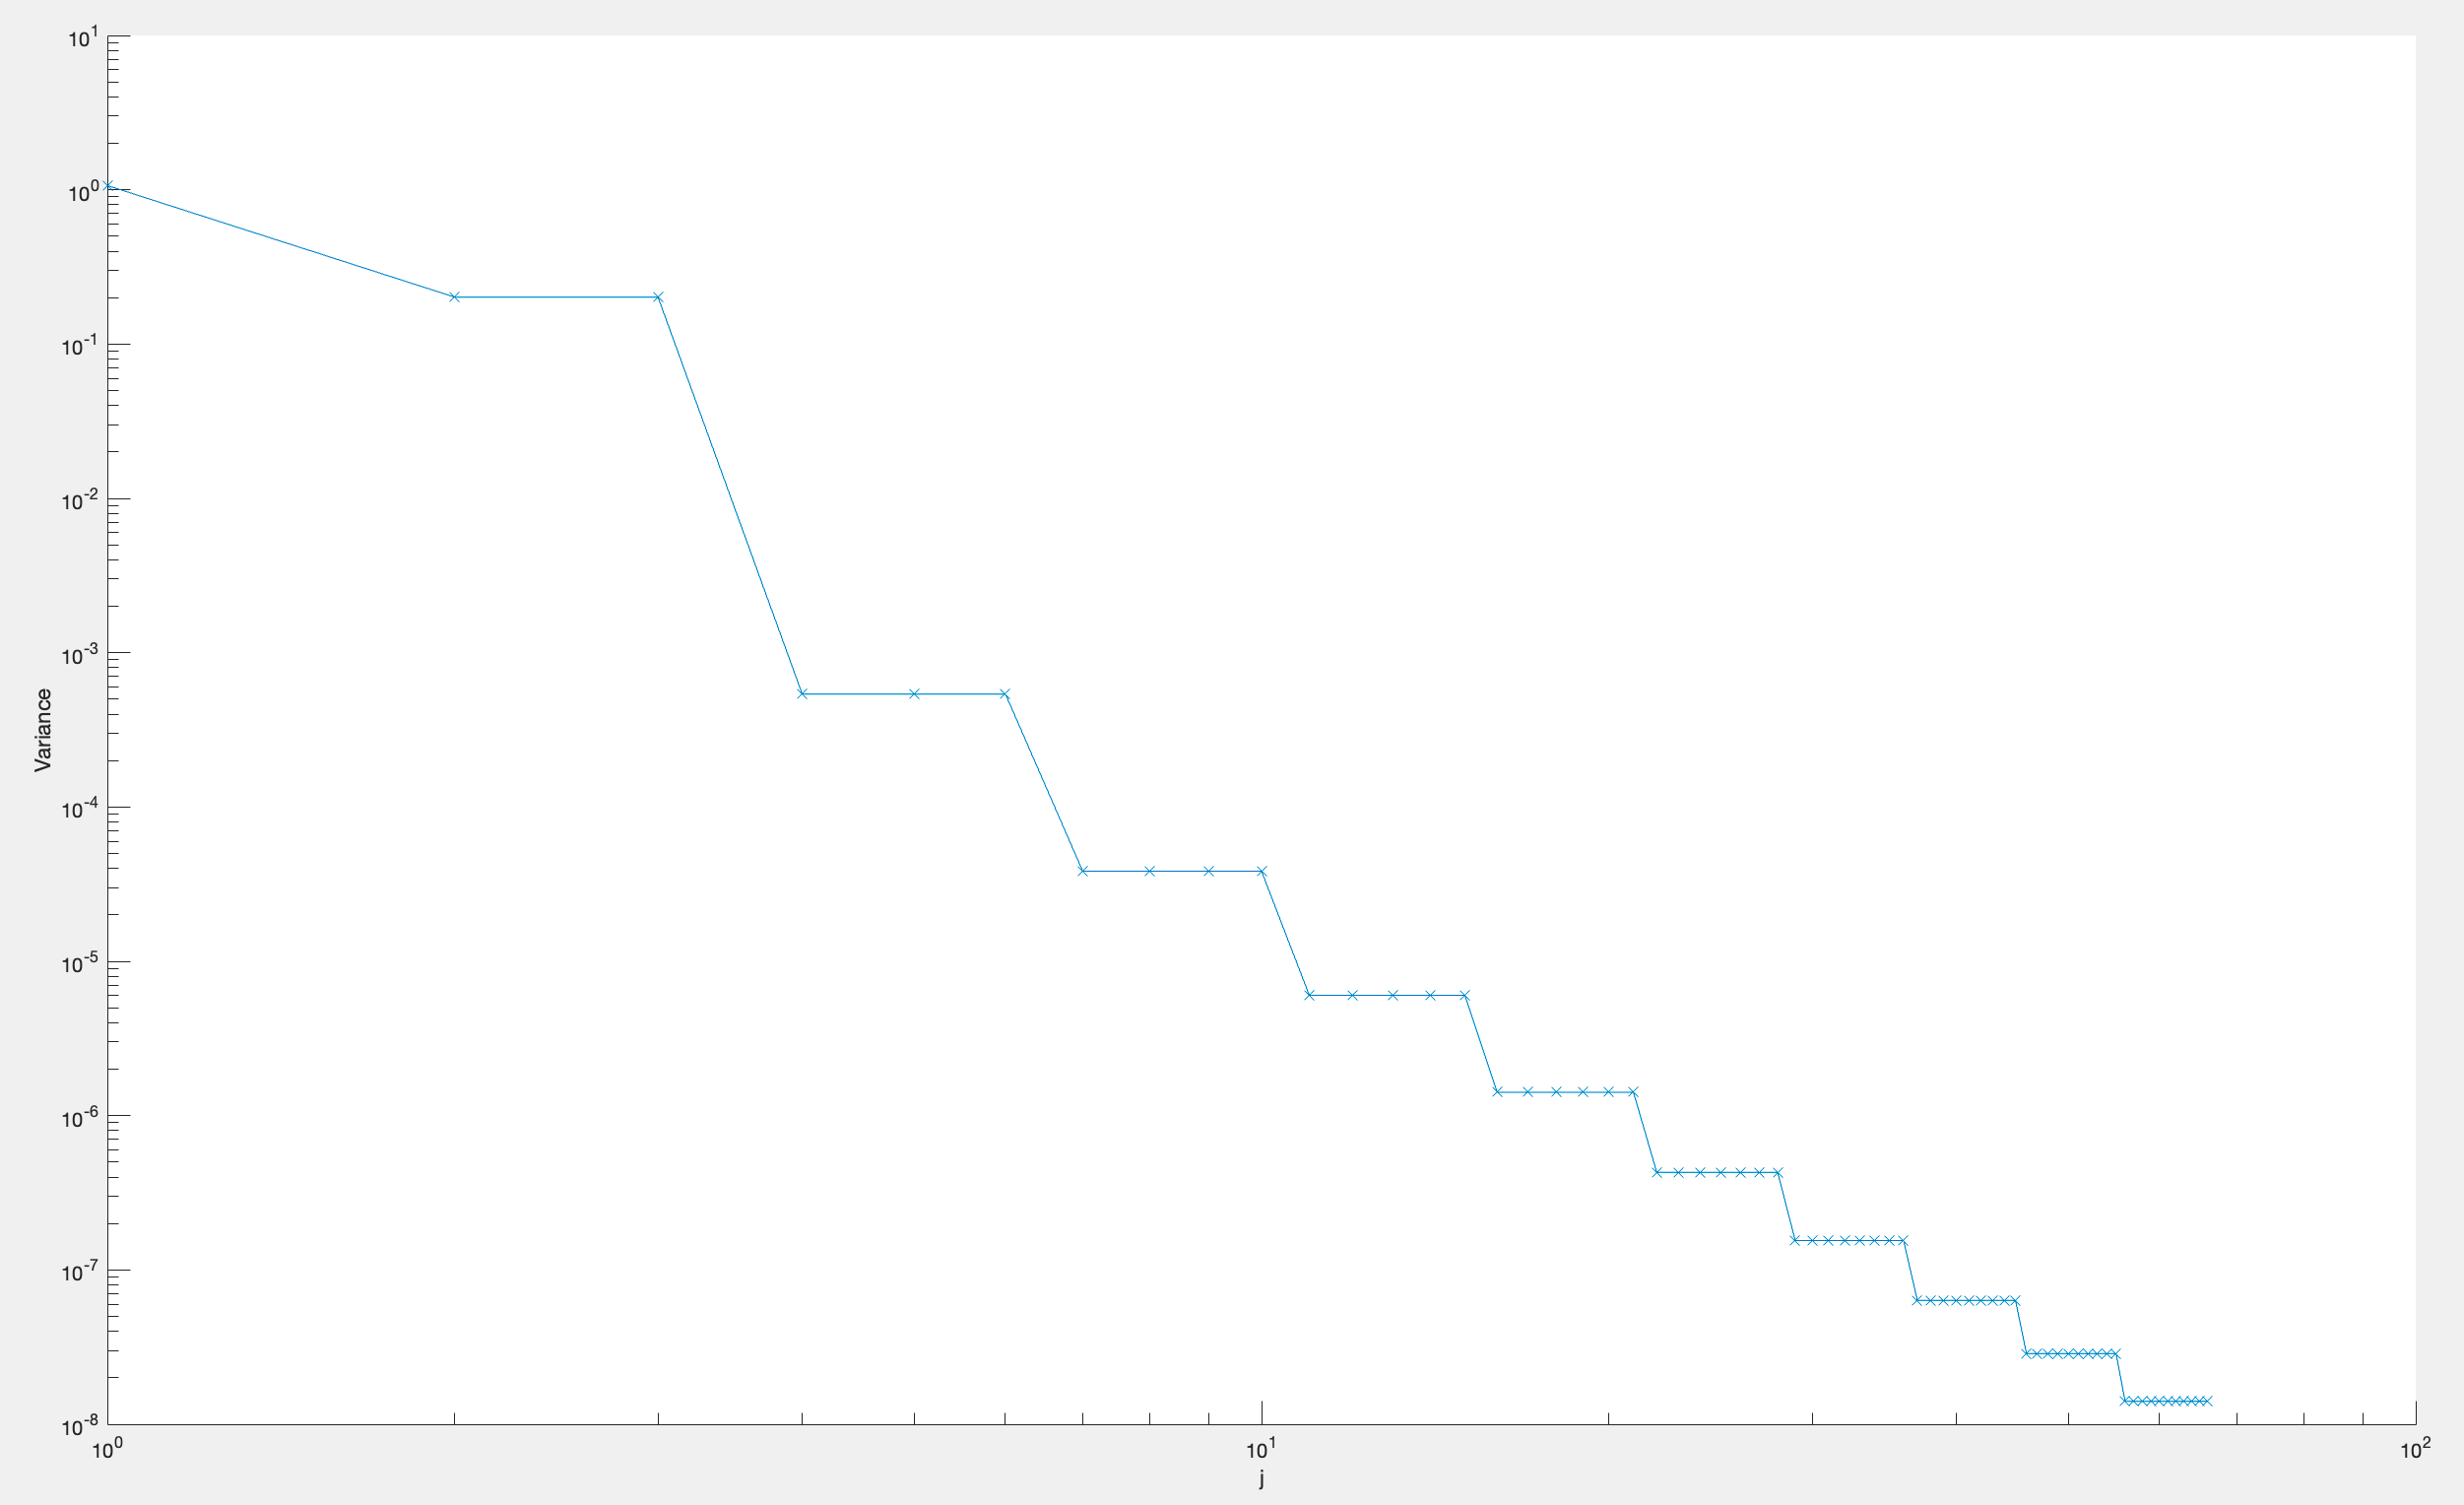
\includegraphics[width = 0.7\textwidth]{assets/figures/mesures/plot_variance_Noll.png}
    \caption{Plot des variances de Noll}
\end{figure}
Ce plot est l'allure typique que nos mesures devraient suivre. Il représente les variances des coefficients de Zernike
des turbulences atmosphériques.

\newpage
Comme dit dans la théorie, selon l'\autoref{eq:param_fried}, convient maintenant de trouver le paramètre de Fried $r_0$
pour faire correspondre au mieux la courbe des mesures de l'écran et celle des valeurs théoriques :
\begin{figure}[H]
    \centering
    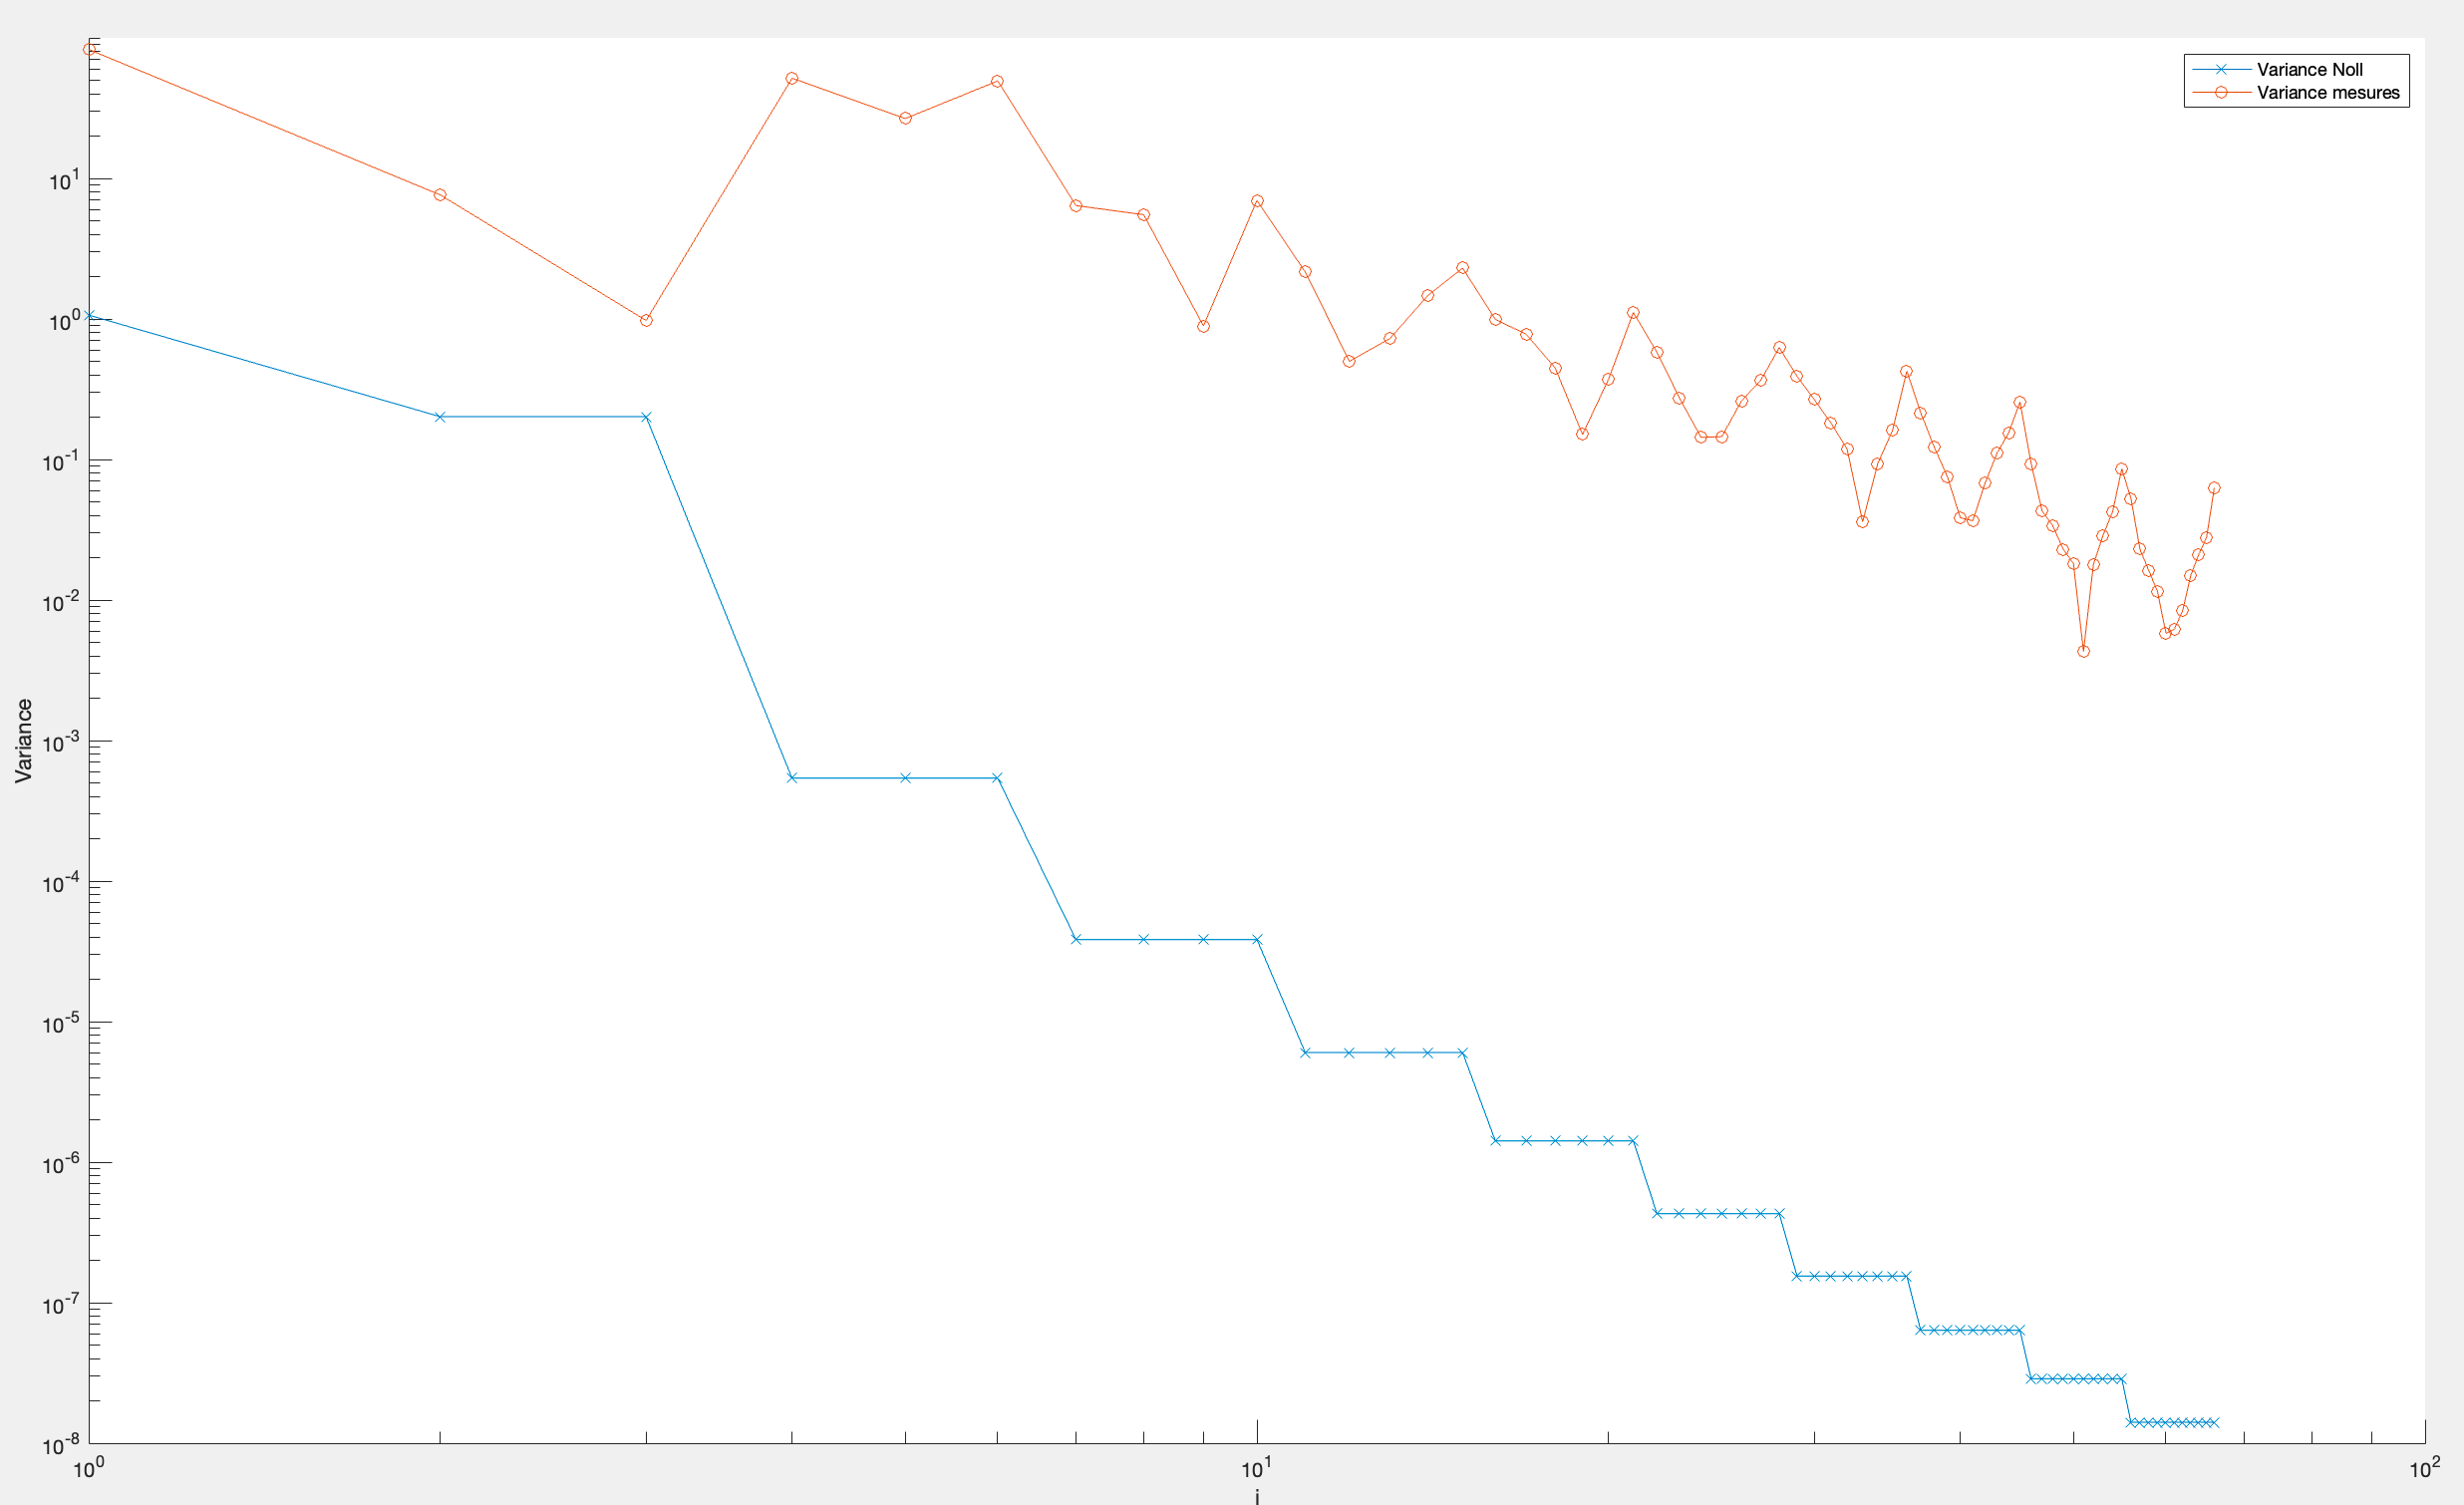
\includegraphics[width = 0.7\textwidth]{assets/figures/mesures/Noll_vs_mesure.png}
    \caption{Plot des variances de Noll vs Variance mesures}
\end{figure}

Pour se faire il conviendra de d'utiliser les fonctions \textit{fittype} et \textit{fit} pour trouver le $r_0$ qui convient le mieux :
\begin{figure}[H]
    \centering
    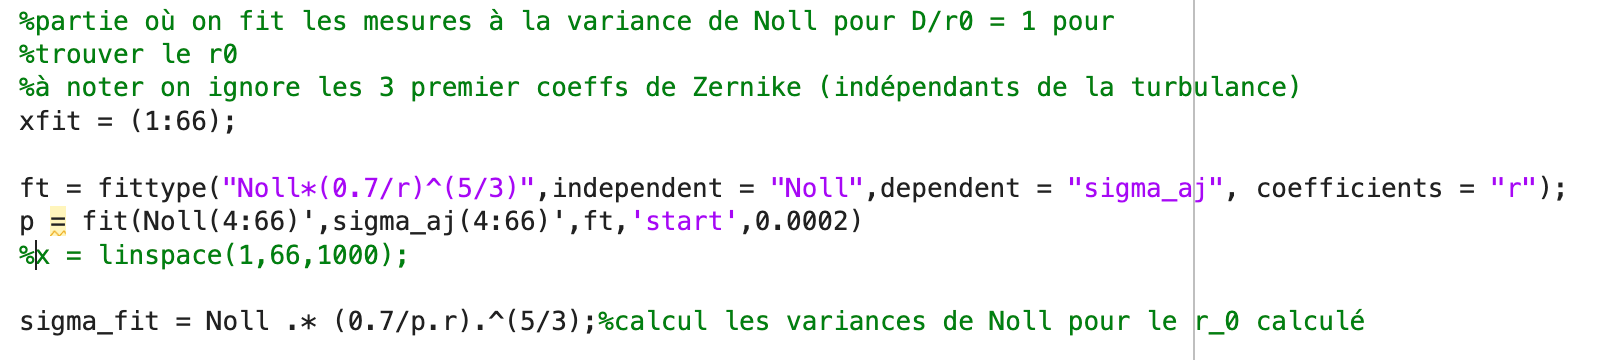
\includegraphics[width = 0.7\textwidth]{assets/figures/mesures/matlab_fit.png}
    \caption{Ligne du script pour fit le $r_0$}
\end{figure}
\color{red}/!\textbackslash \color{black}Dans le fit on exlu les 3 premiers coefficients de Zernike (Piston, inclinaison verticale, inclinaison horizontale),
en effet, ces 3 coefficients ne sont pas influencés par la turbulence mais par le système optique en lui même, ils ne sont donc pas relevant pour le fit.

La ligne commençant par \textbf{sigma\textunderscore fit} utilise l'\autoref{eq:param_fried}, où cette fois-ci on utilise le diamètre du diaphragme du système optique pour la
valeur de \textbf{D} ($\approx0.7 cm$). Une fois le fit effectué, il est possible de voir la valeur trouvée de $r_0$ dans la \textit{Command Window} de Matlab :
\begin{figure}[H]
    \centering
    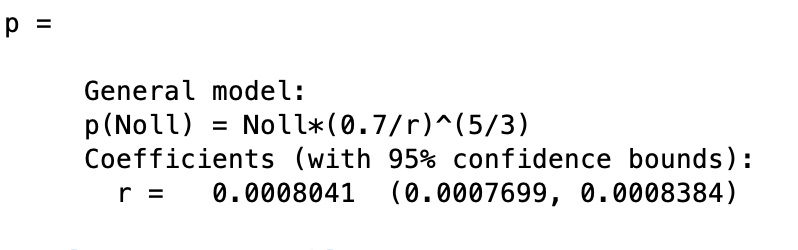
\includegraphics[width = 0.7\textwidth]{assets/figures/mesures/fit_r_resultat.png}
    \caption{Exemple de $r_0$ trouvé par l'algorithme de fit}
\end{figure}

\newpage
Au final, le graph suivant est obtenu :
\begin{figure}[H]
    \centering
    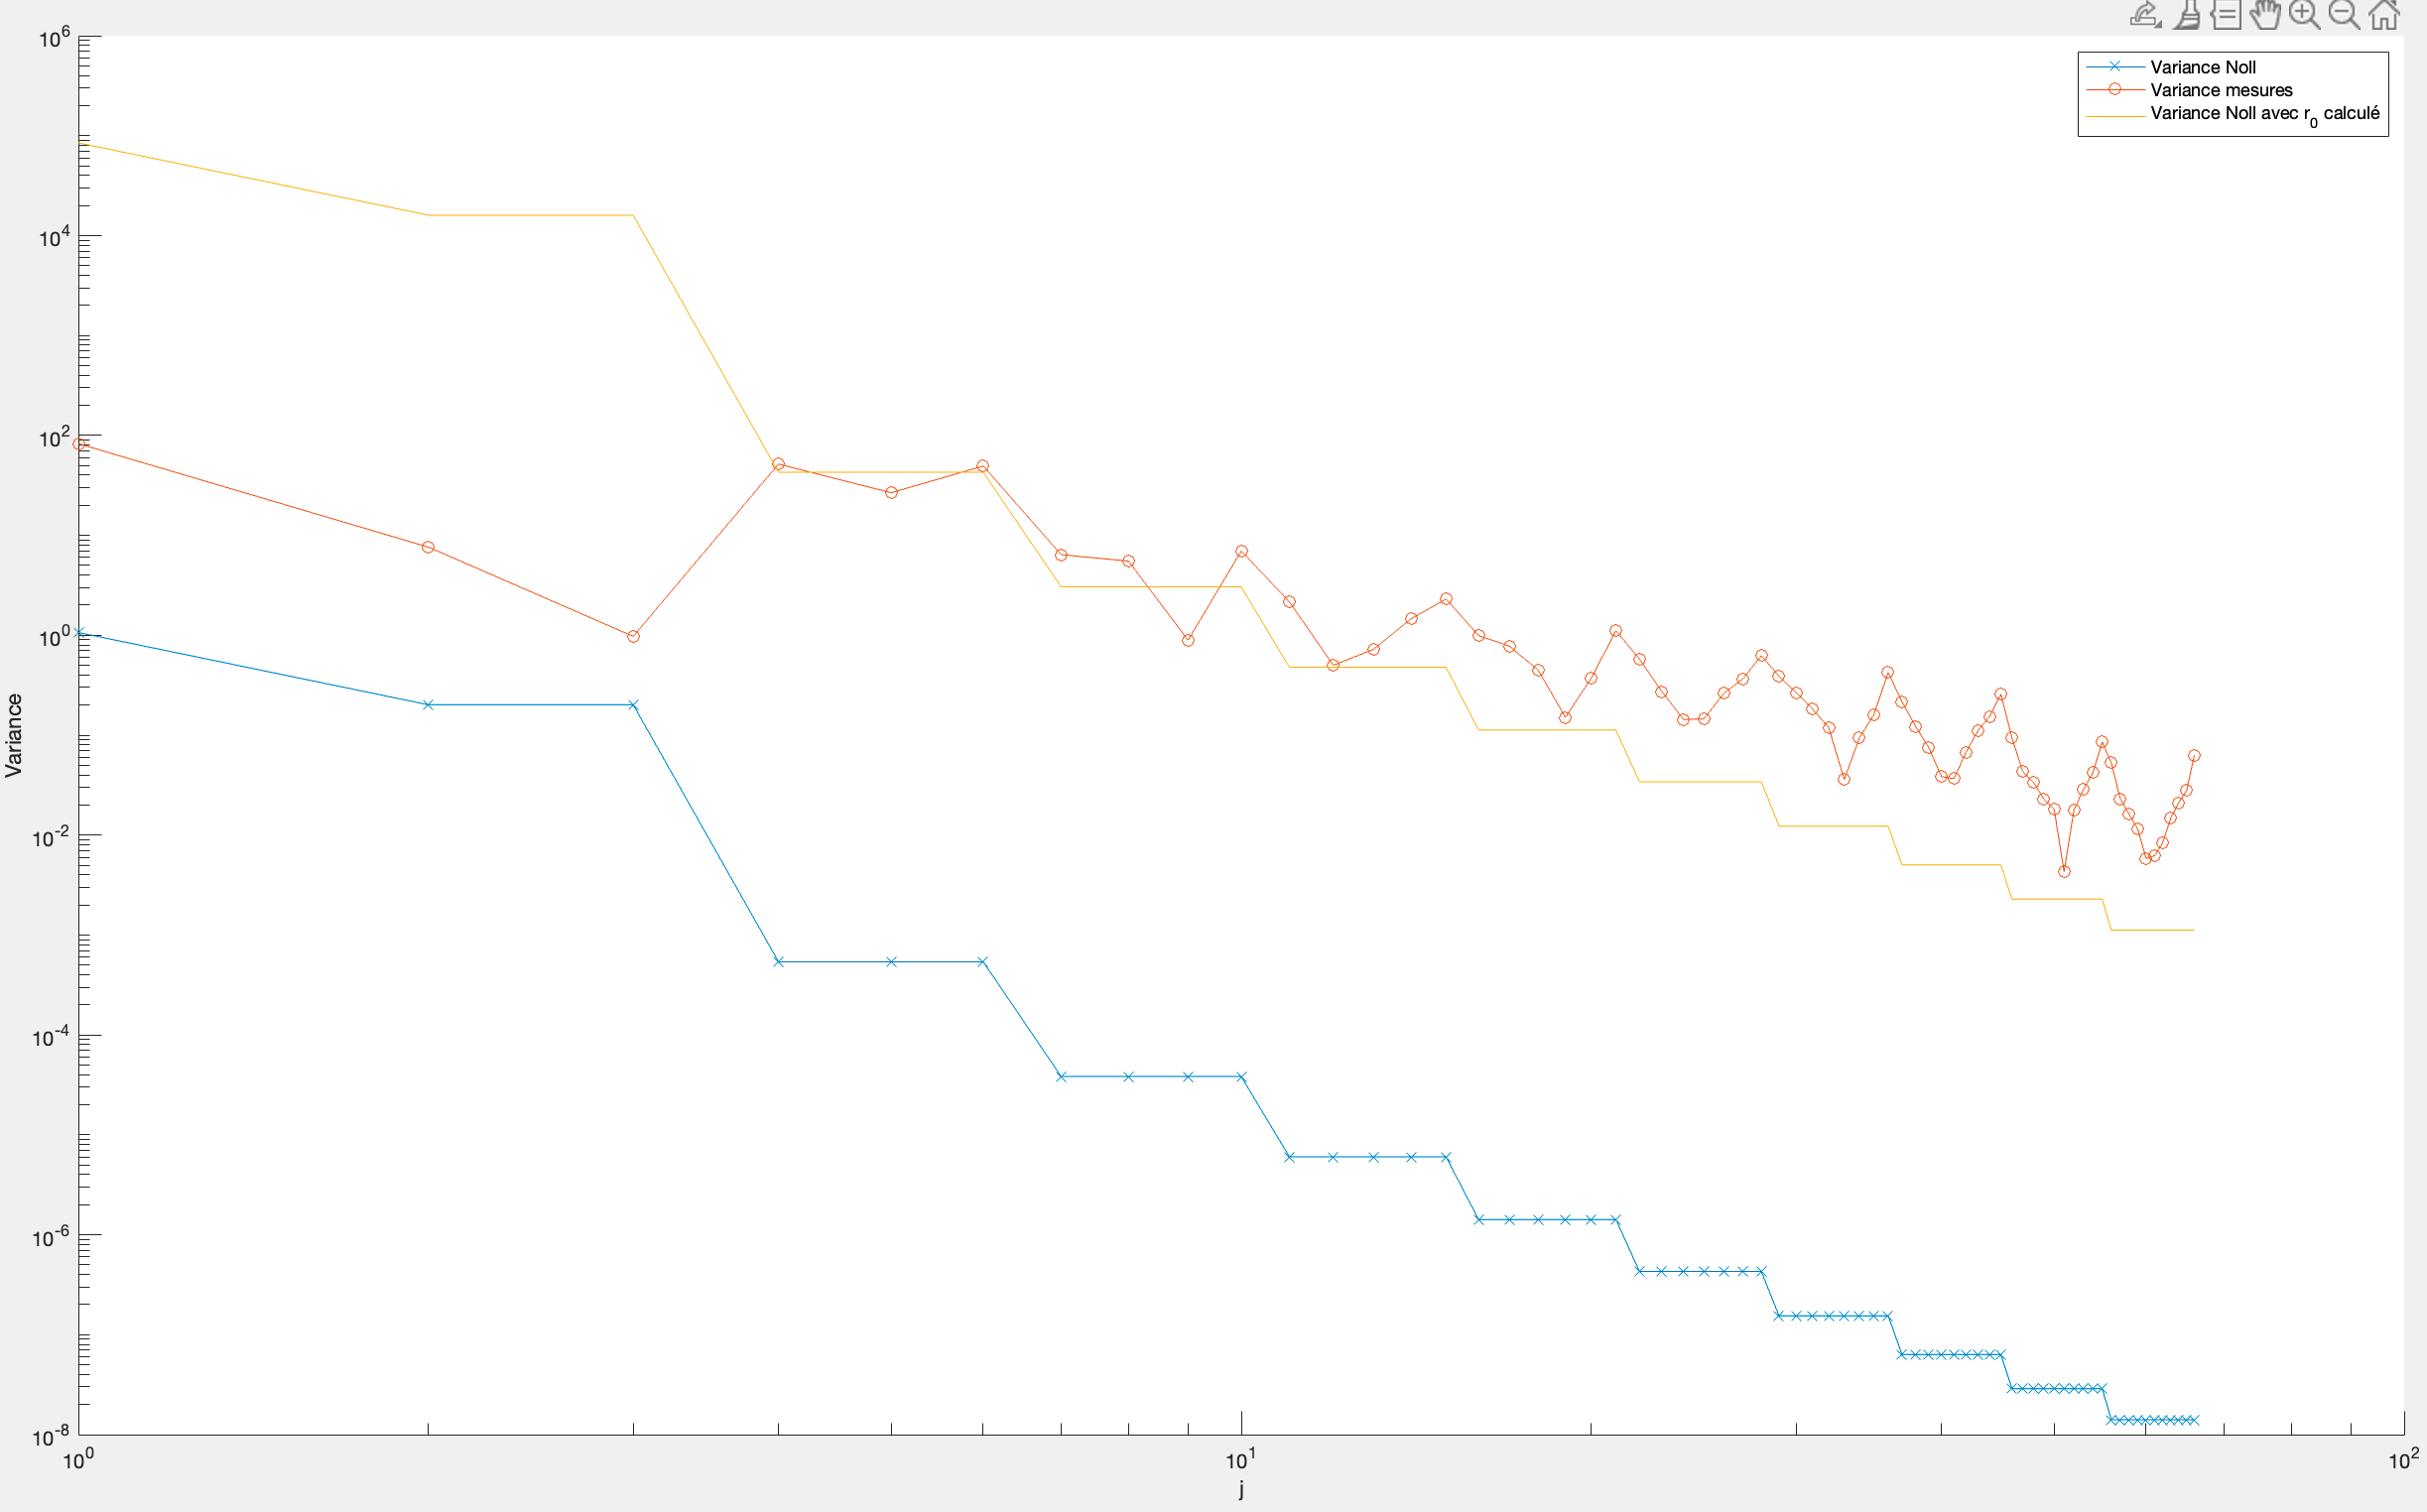
\includegraphics[width = 1\textwidth]{assets/figures/mesures/Plot_final_avec_fit.png}
    \caption{Graph final avec variance Noll, variance mesures et variance fit}
\end{figure}

Dans une deuxième fenêtre, un histogramme de toutes les séries de mesures est affiché pour contrôler la distribution gaussienne de coefficients :
\begin{figure}[H]
    \centering
    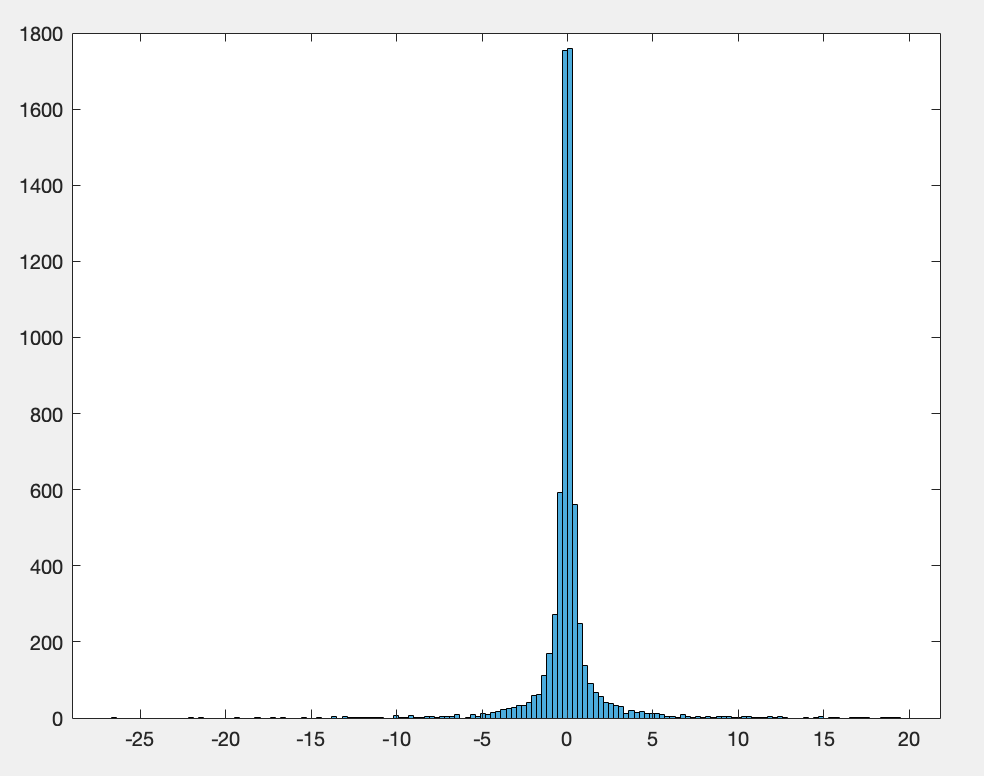
\includegraphics[width = 0.6\textwidth]{assets/figures/mesures/histogramme_mesure.png}
    \caption{Histogramme de contrôle de la répartition des mesures}
\end{figure}

Le code du scipt d'analyse est disponible dans la \autoref{code:script_mesure_matlab}.

\newpage
\section{Résultats}
\subsection{Écran 15 secondes}
Plusieurs séries de mesures fûrent réalisées pour l'écran de 15 secondes :
\begin{figure}[H]
    \centering
    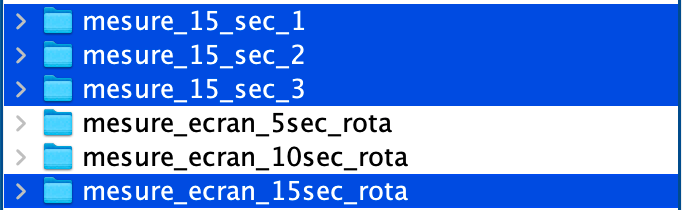
\includegraphics[width = 0.6\textwidth]{assets/figures/mesures/series_mesures_15sec.png}
    \caption{Séries de mesures écran 15 secondes}
\end{figure}
Les 3 premières séries ont étées réalisées à la suite avec les paramètres suivants :
\begin{itemize}
    \item Angle rotation : 3.6\textdegree
    \item Translation : 0mm
    \item Nombre de mesures : 100
\end{itemize}
Donc chaque séries se passe à exactement la même distance horizontale, commence et se finit à la même position angulaire.

La dernière série de mesure a été réalisée plus tôt pour tester le système de mesure.

\subsubsection{Mesure 15 secondes 1}
\begin{figure}[H]
    \centering
    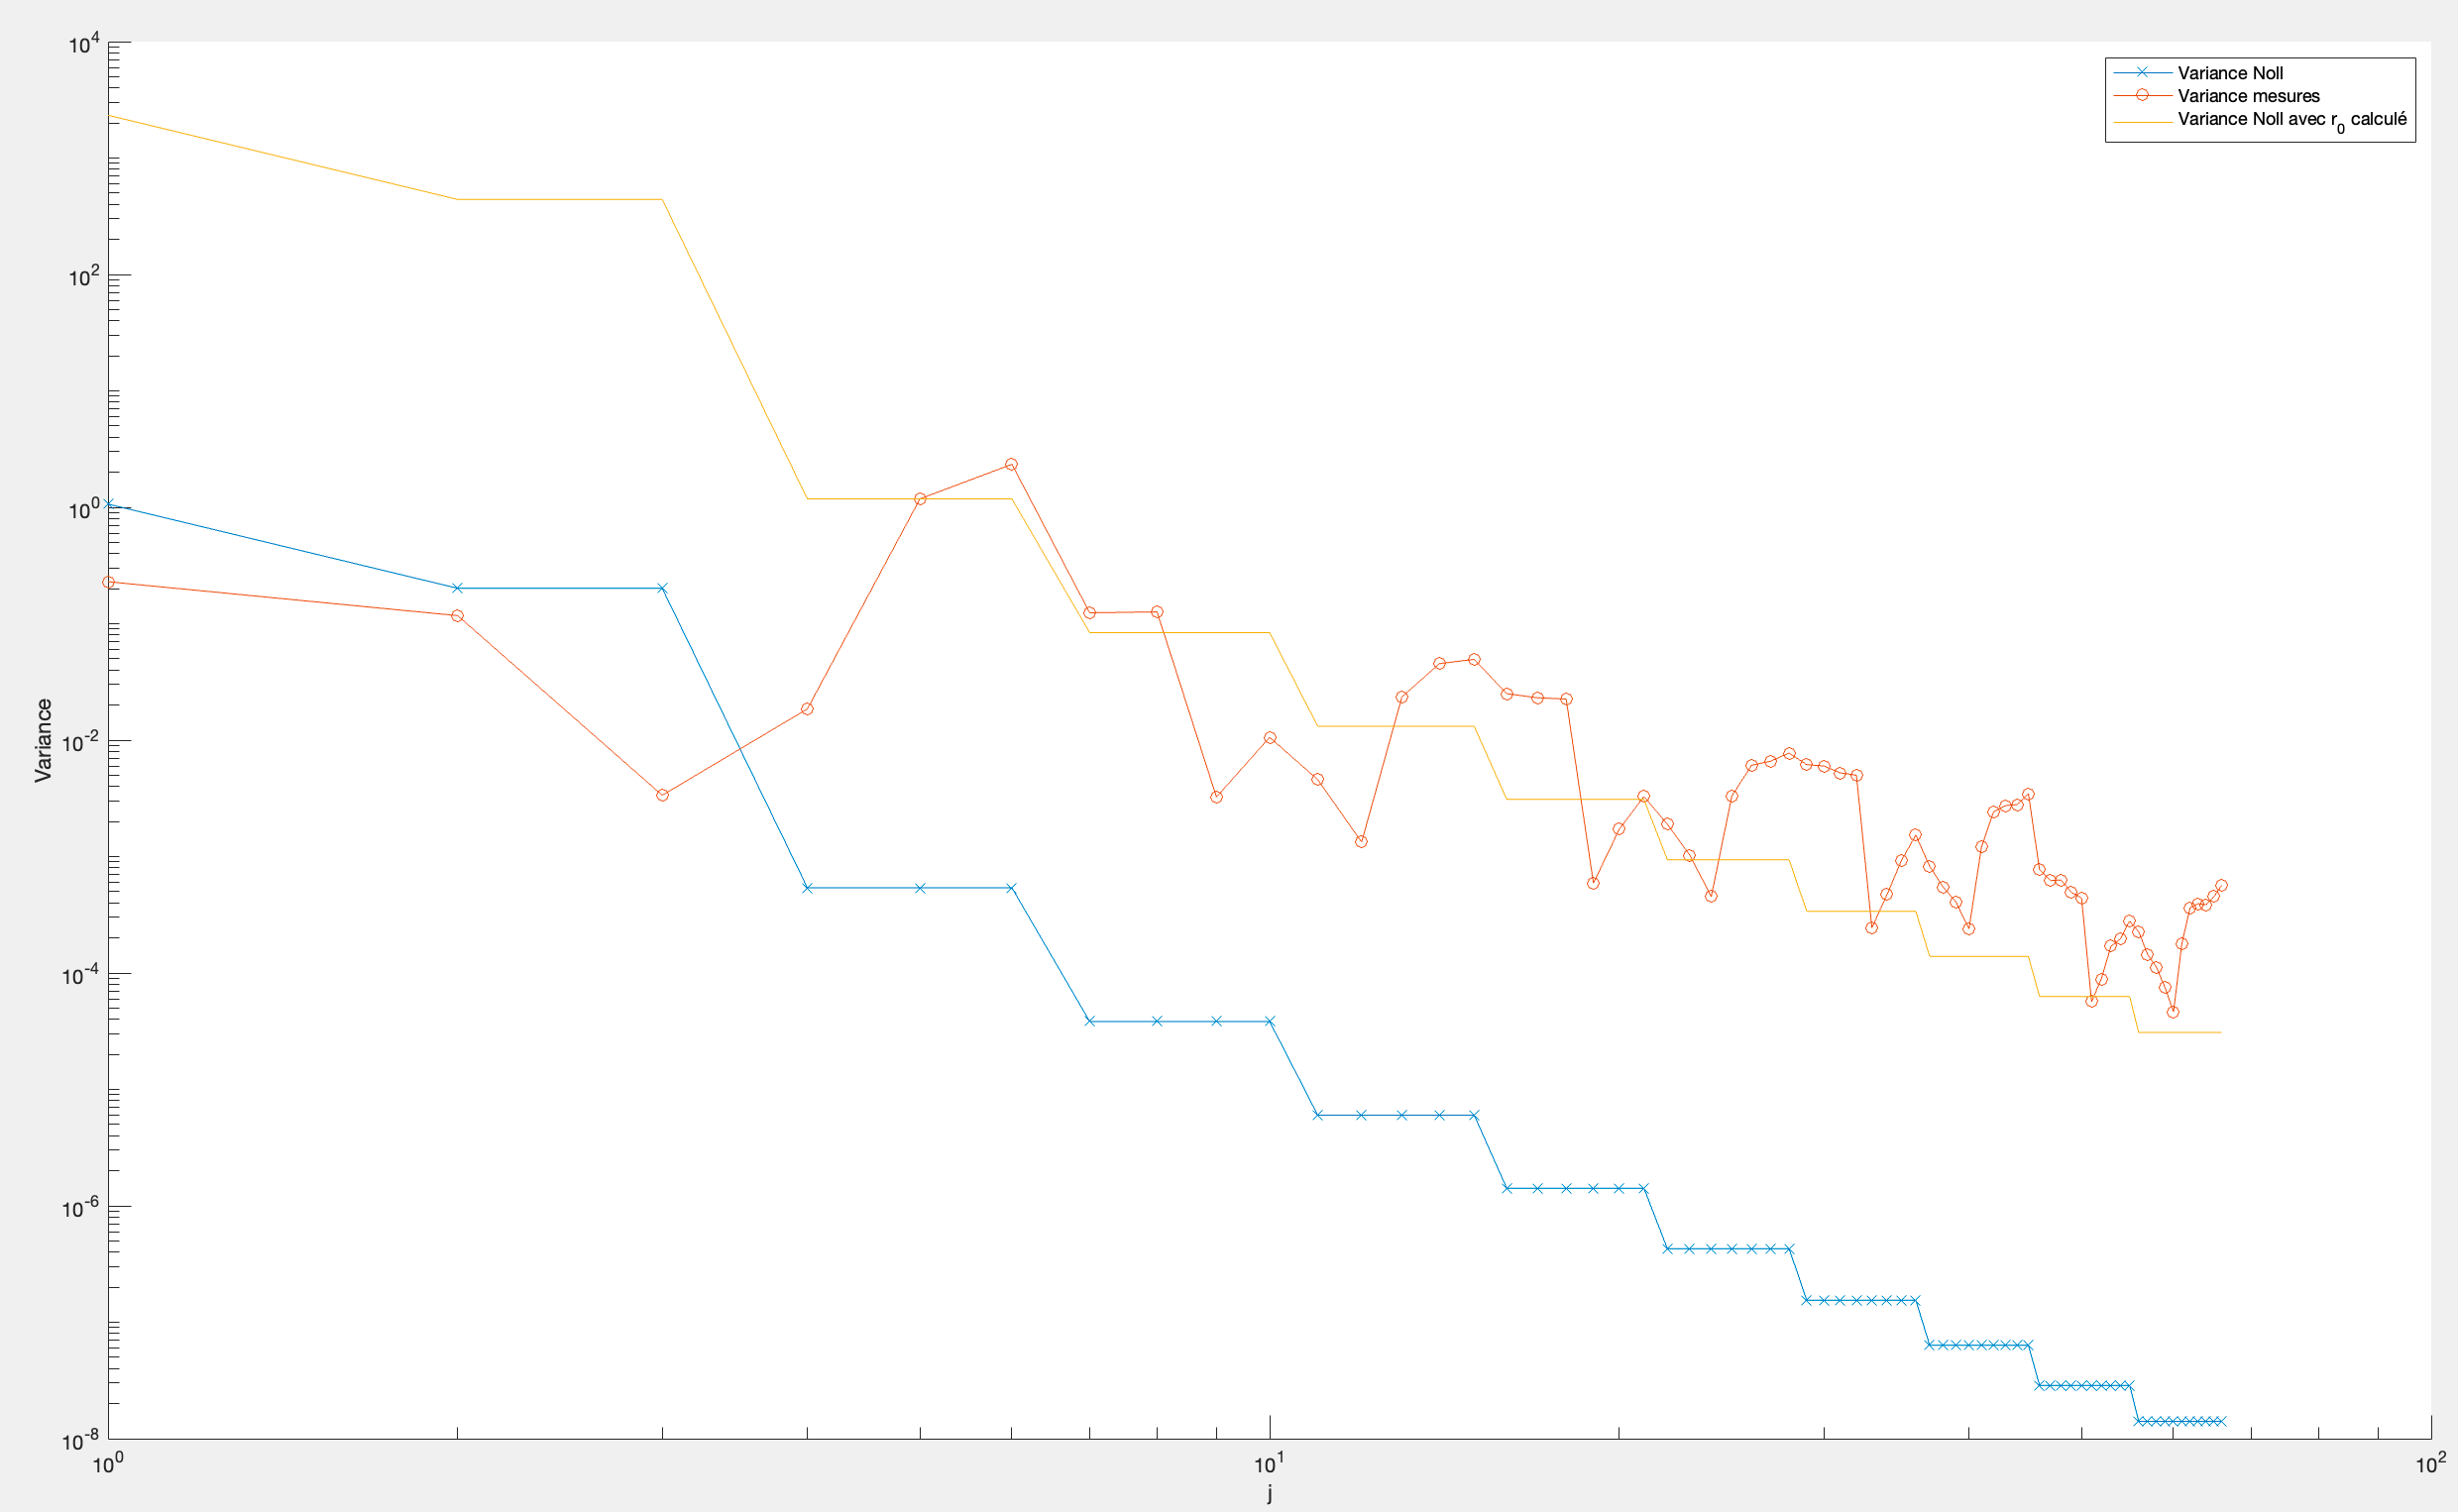
\includegraphics[width = \textwidth]{assets/figures/mesures/mesure_15_sec_1_plot.png}
    \caption{Graphique de la série consécutive 1}
\end{figure}
Le \textbf{$r_0$} calculé est égal à : \textbf{0.006937 cm}.

\subsubsection{Mesure 15 secondes 2}
\begin{figure}[H]
    \centering
    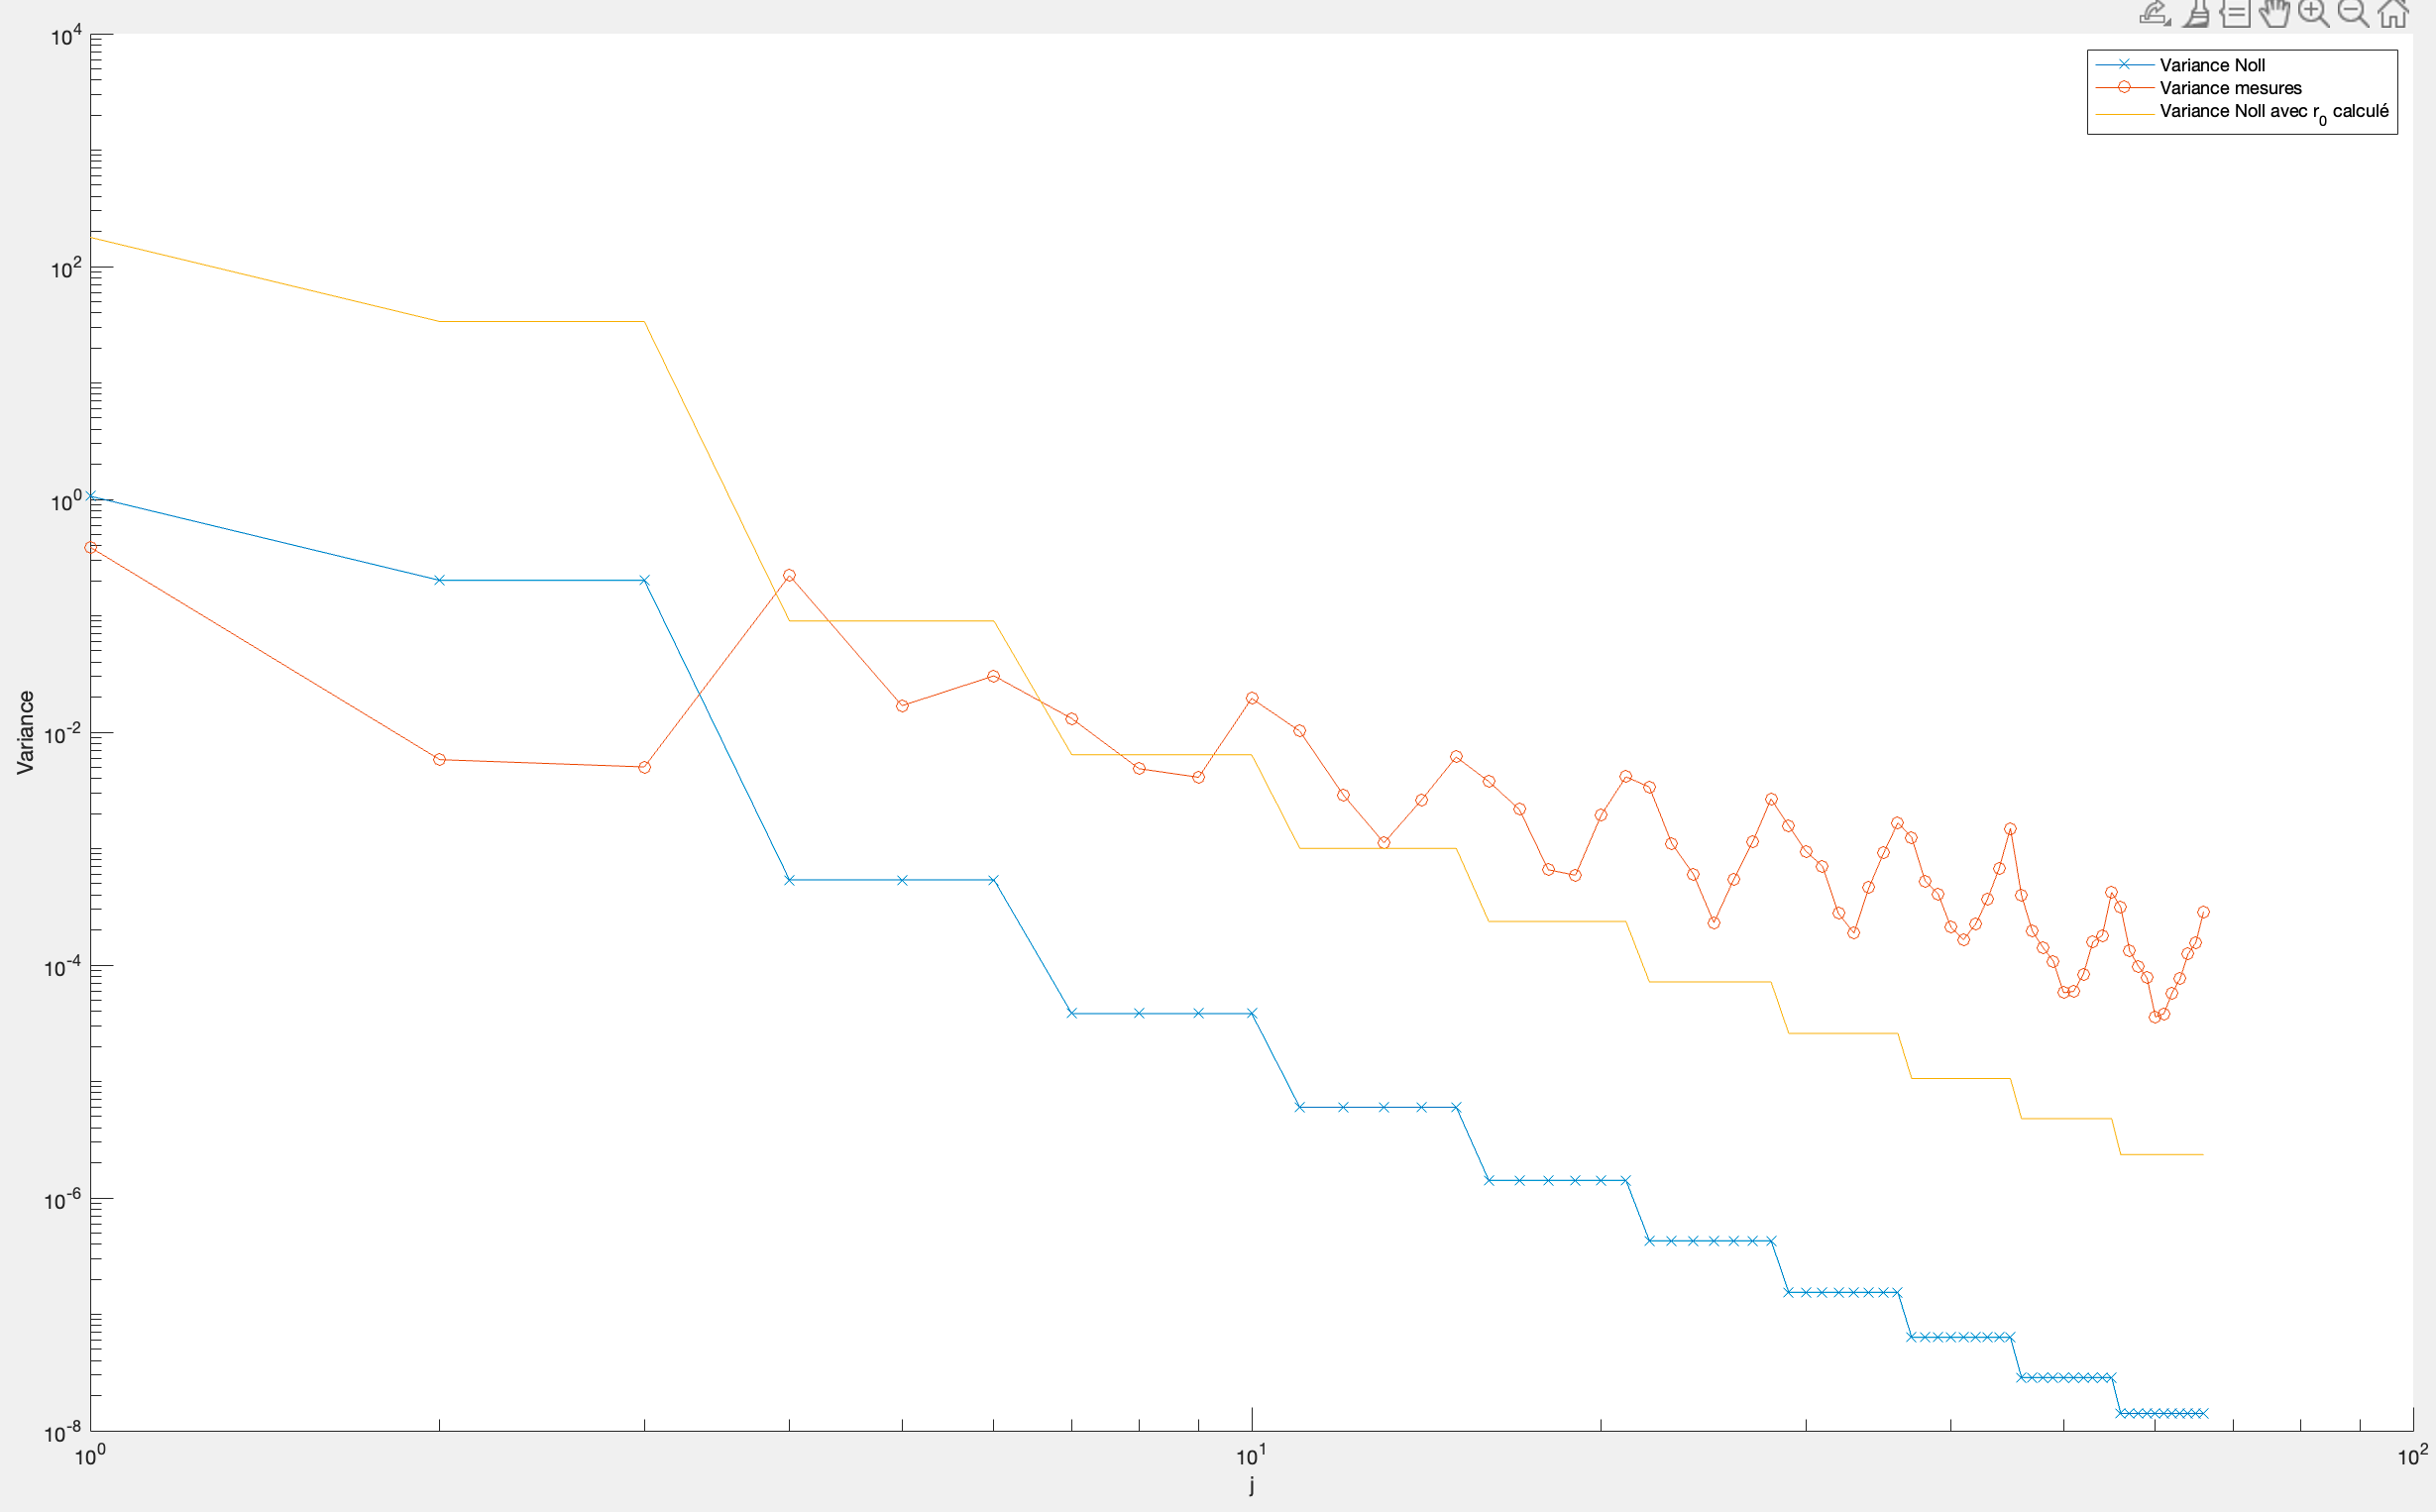
\includegraphics[width = \textwidth]{assets/figures/mesures/mesure_15_sec_2_plot.png}
    \caption{Graphique de la série consécutive 2}
\end{figure}
Le \textbf{$r_0$} calculé est égal à : \textbf{0.03245 cm}.

\subsubsection{Mesure 15 secondes 3}
\begin{figure}[H]
    \centering
    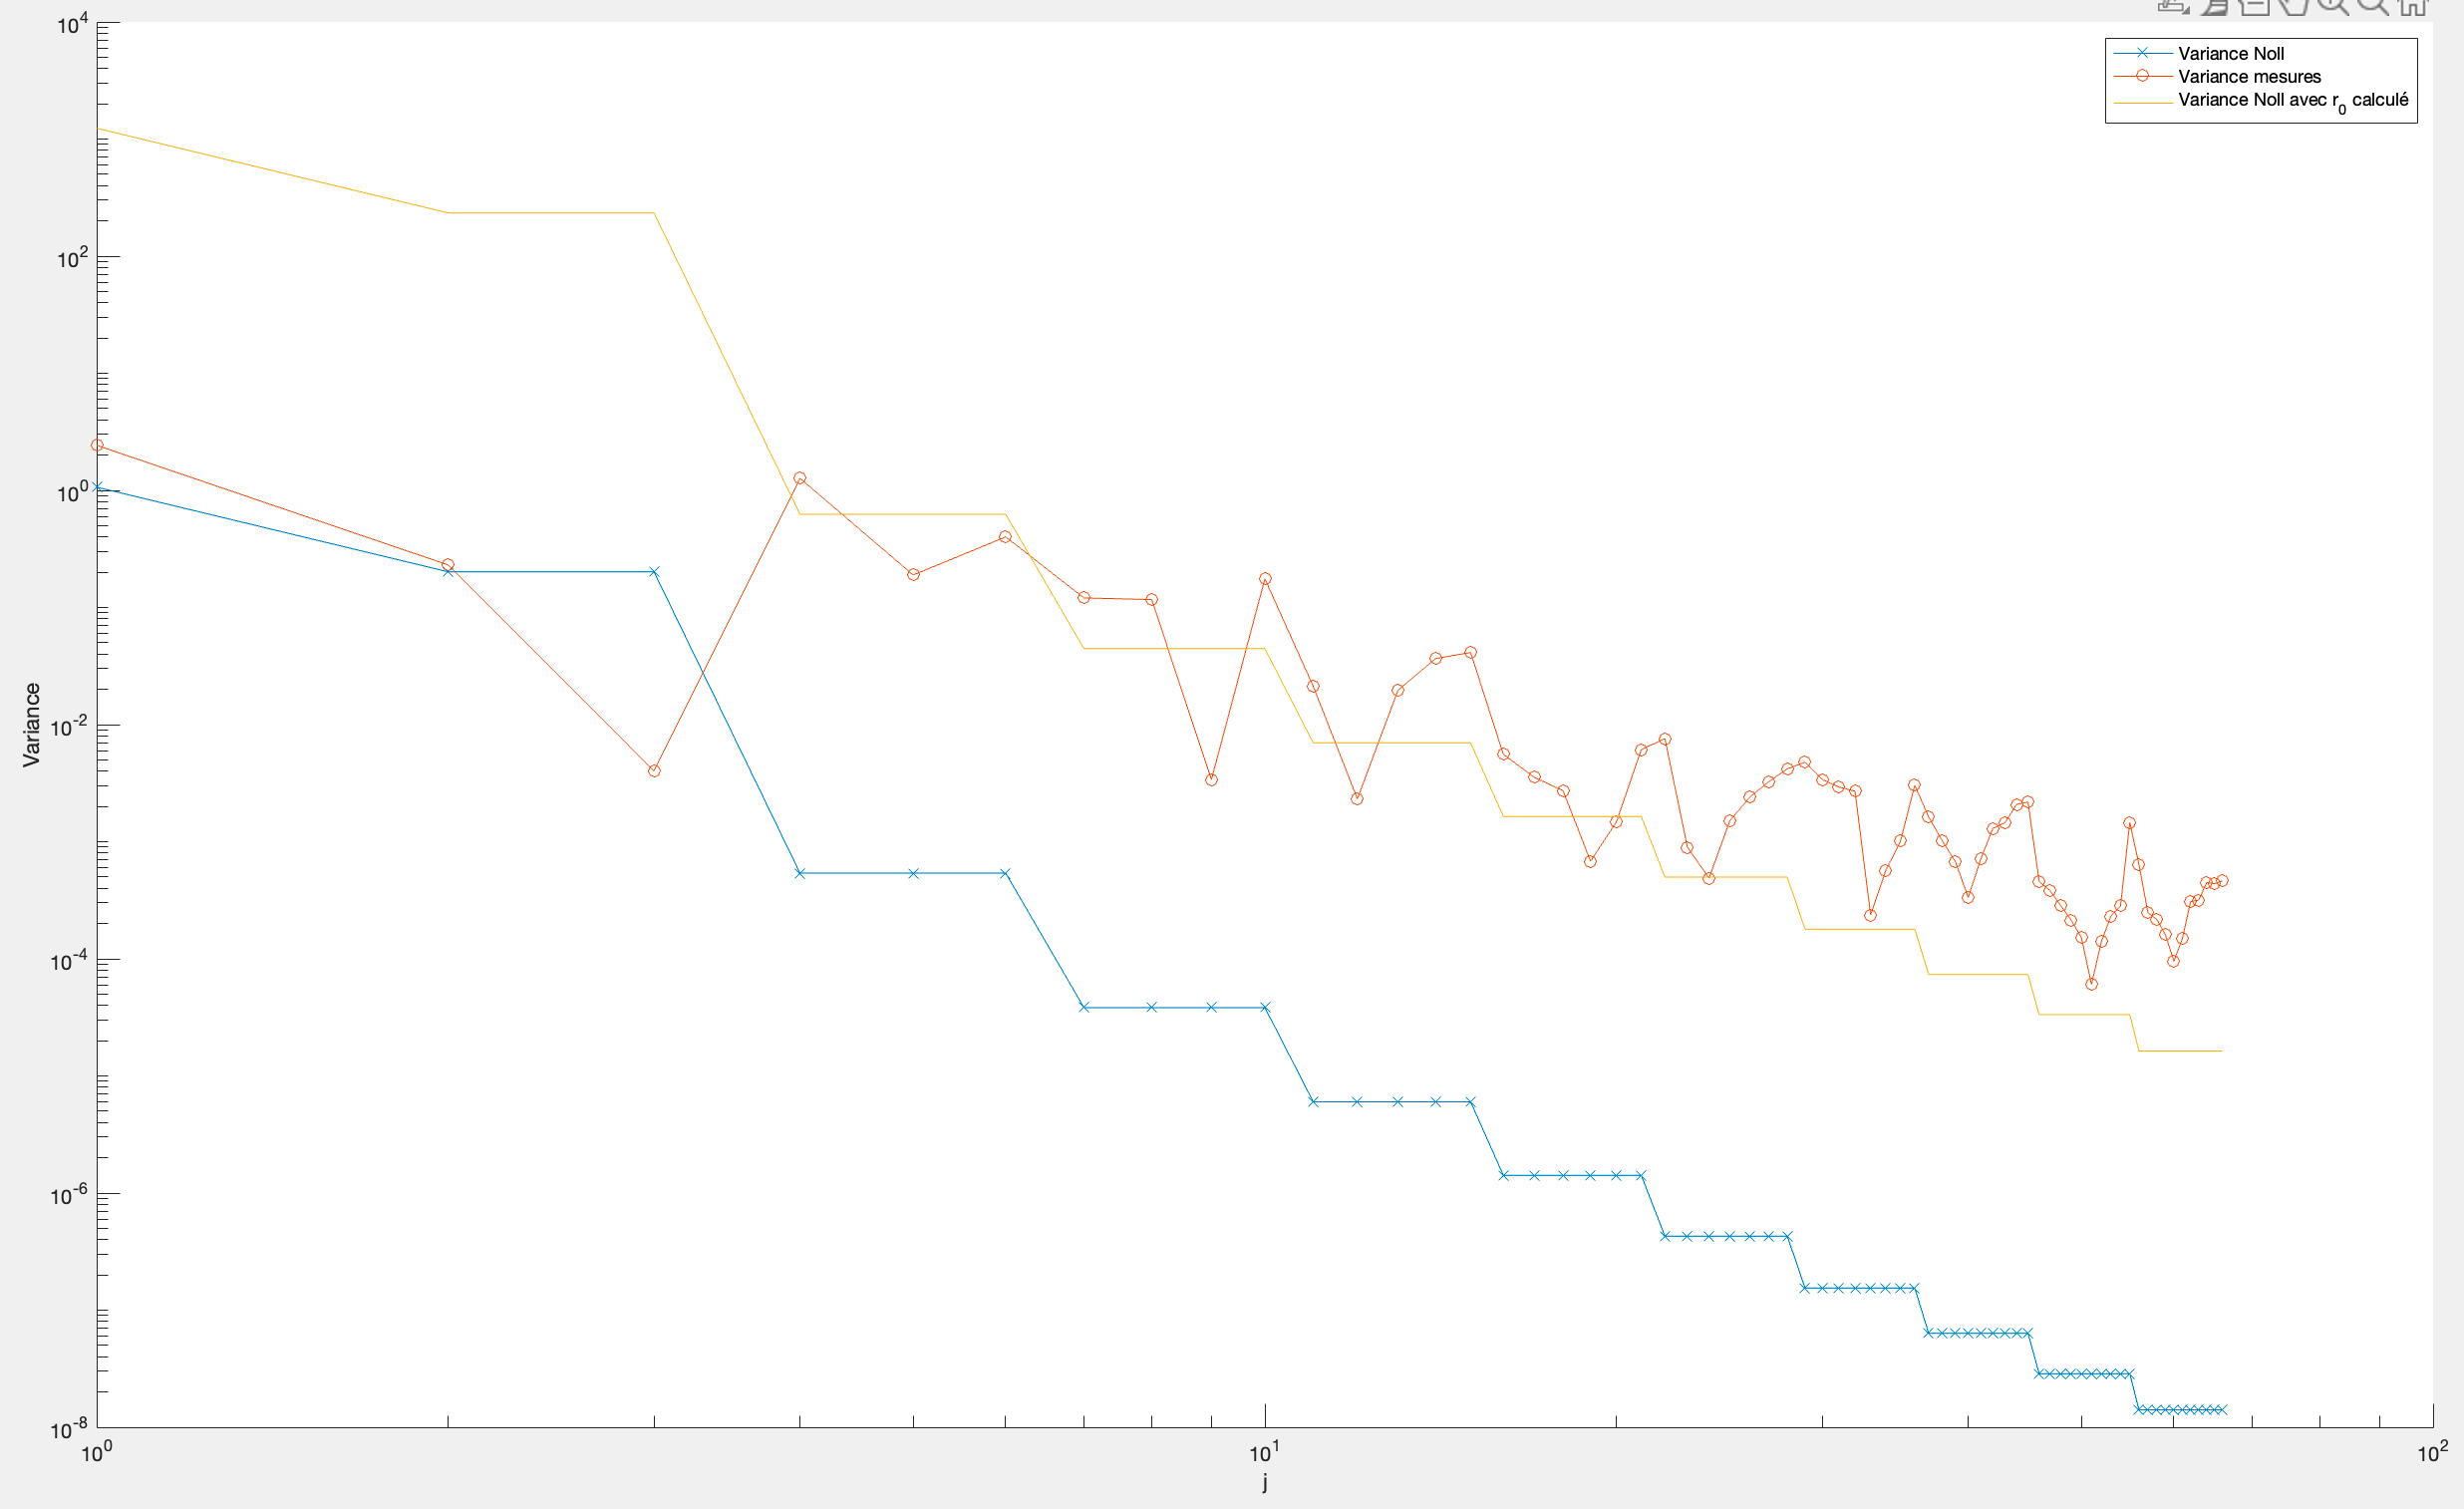
\includegraphics[width = \textwidth]{assets/figures/mesures/mesure_15_sec_3_plot.png}
    \caption{Graphique de la série consécutive 3}
\end{figure}
Le \textbf{$r_0$} calculé est égal à : \textbf{0.01015 cm}.

\subsubsection{Mesure 15 secondes "écran\textunderscore15sec\textunderscore rota"}
\begin{figure}[H]
    \centering
    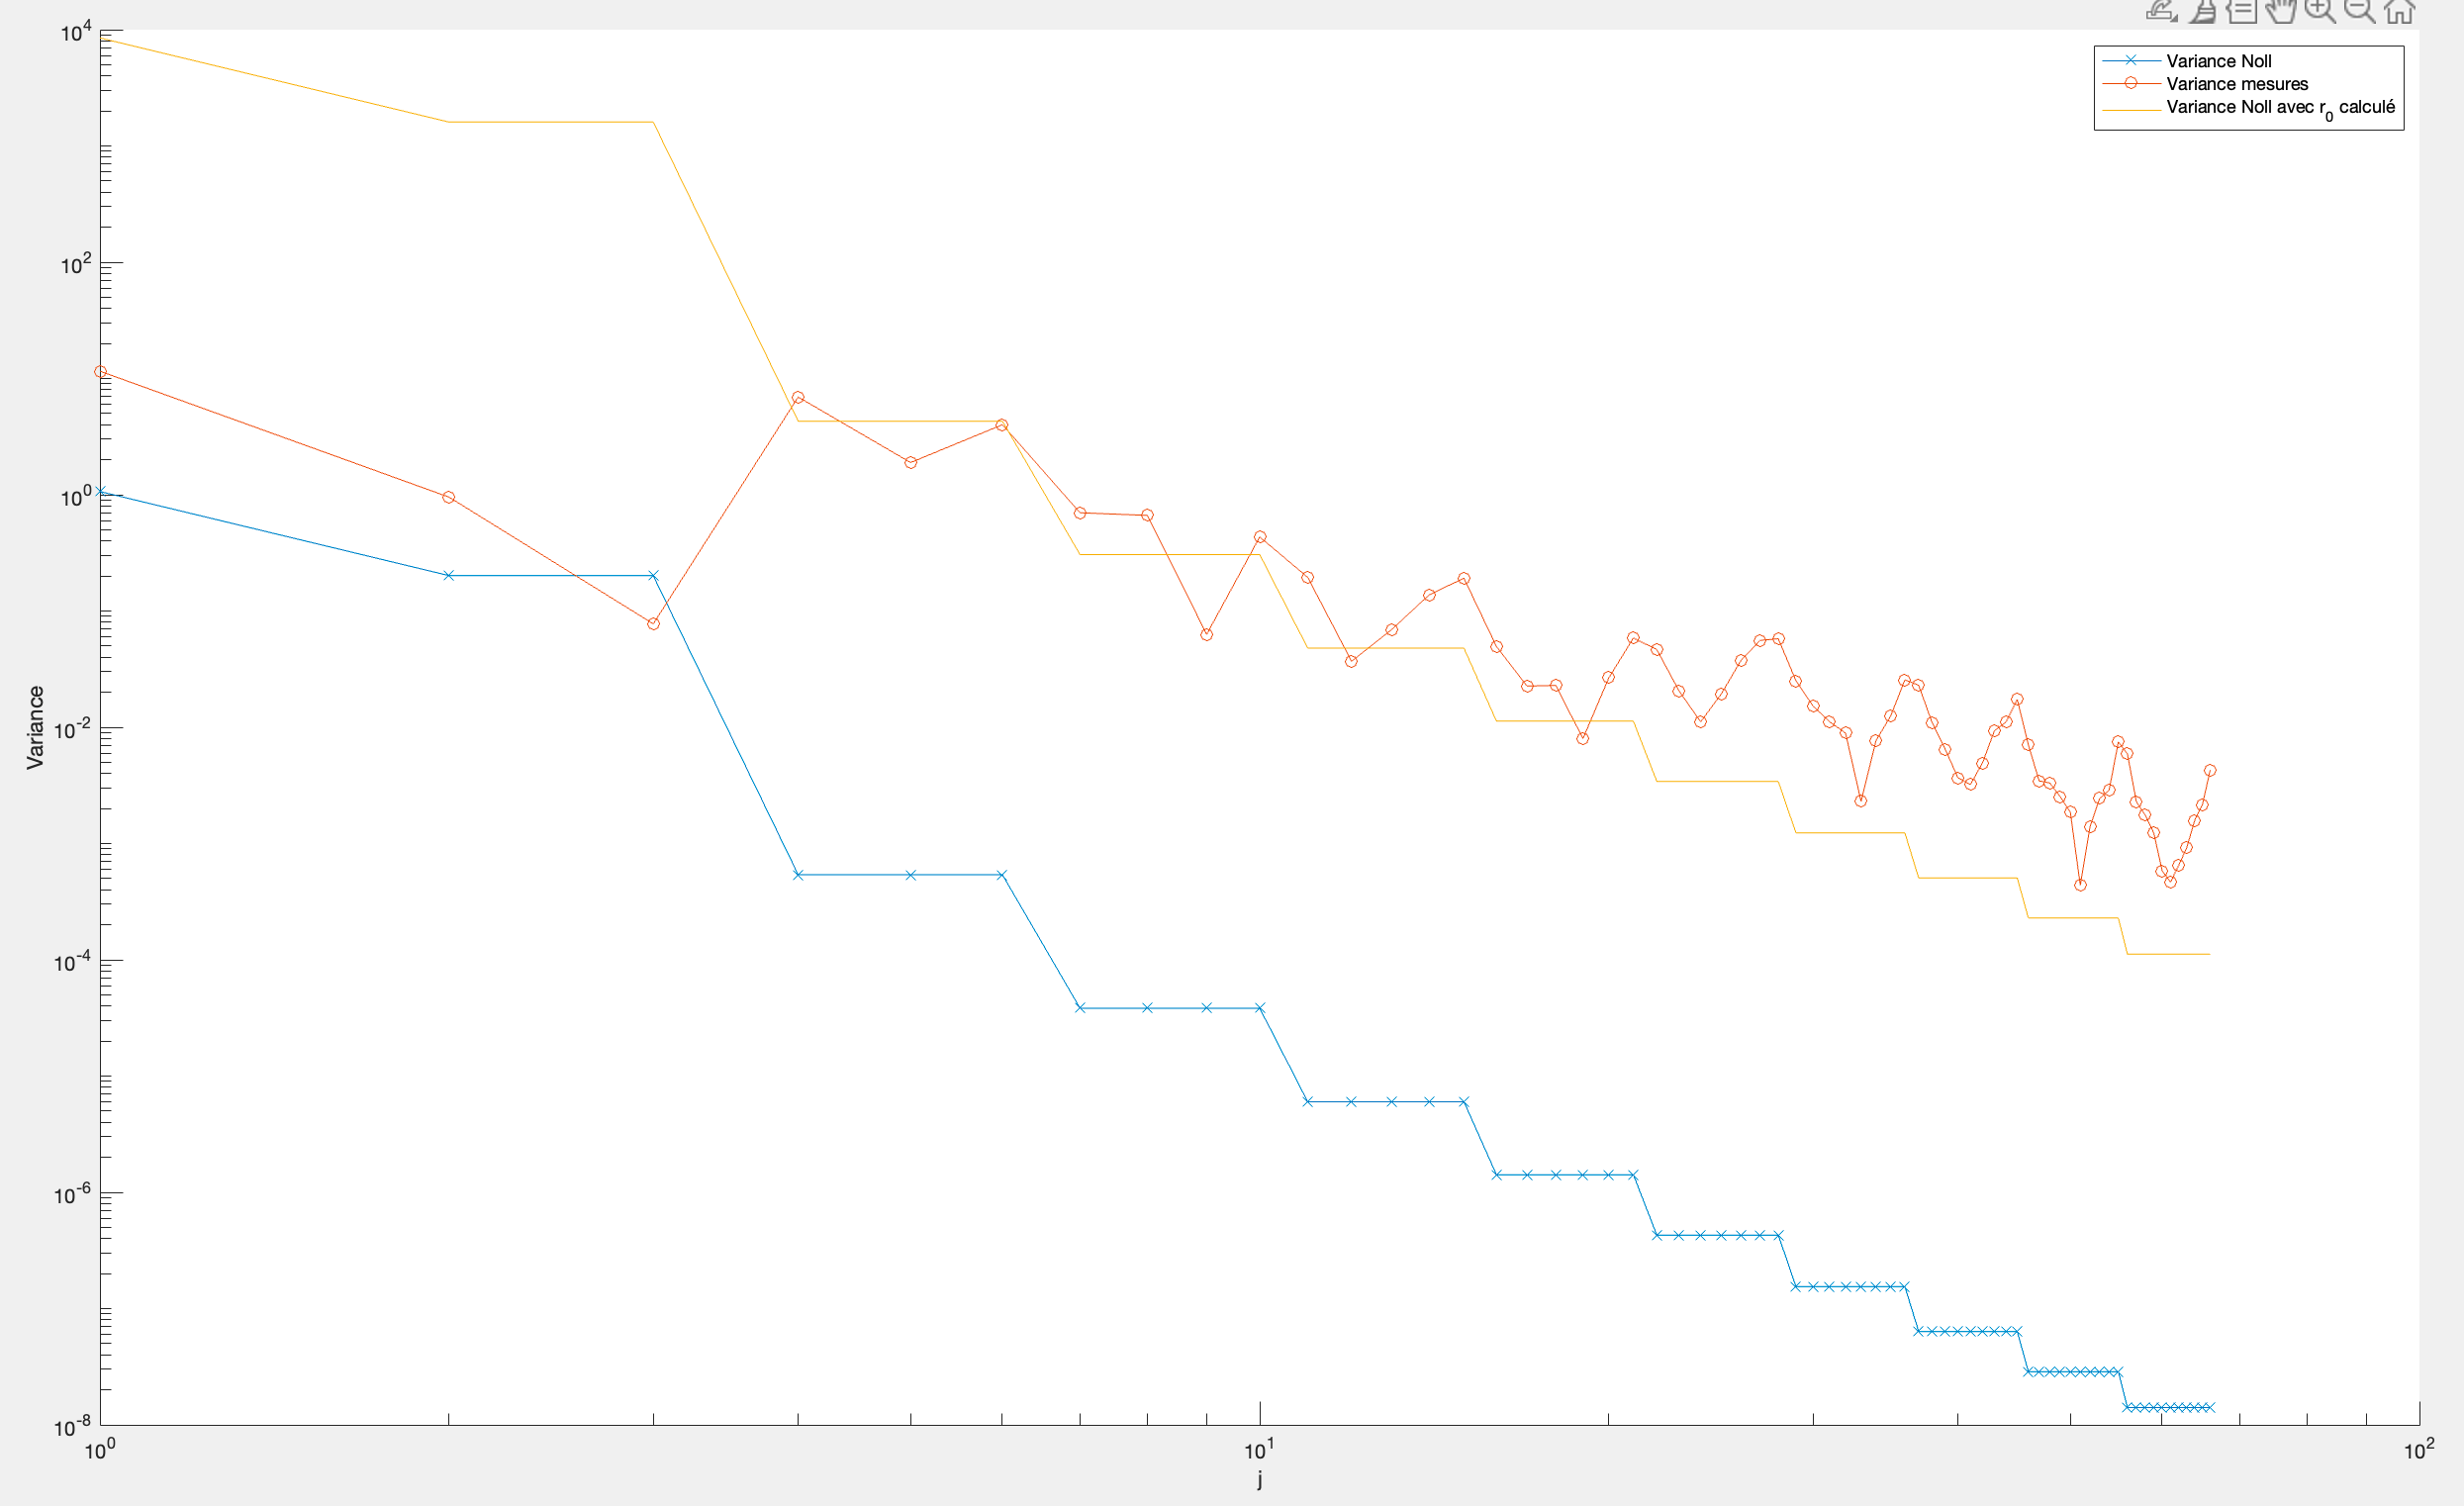
\includegraphics[width = \textwidth]{assets/figures/mesures/mesure_15_sec_rota_plot.png}
    \caption{Graphique de la série "écran\textunderscore15sec\textunderscore rota"}
\end{figure}
Le \textbf{$r_0$} calculé est égal à : \textbf{0.003195 cm}.

\subsection{Écran 30 secondes}
Ici une seule série de mesures avec les même paramètres que les écrans de 15 secondes a été réalisée :
\begin{figure}[H]
    \centering
    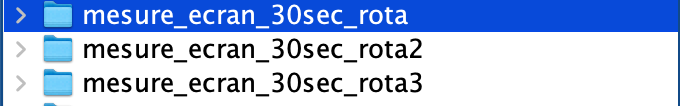
\includegraphics[width = 0.6\textwidth]{assets/figures/mesures/serie_mesures_30_sec_1.png}
    \caption{Série de mesures écran 30 secondes}
\end{figure}
Les deux autres séries ne contiennent que 10 mesures, ce qui n'est pas vraiment significatif pour tirer des conclusions.

\subsubsection{Mesure 30 secondes 1}
\begin{figure}[H]
    \centering
    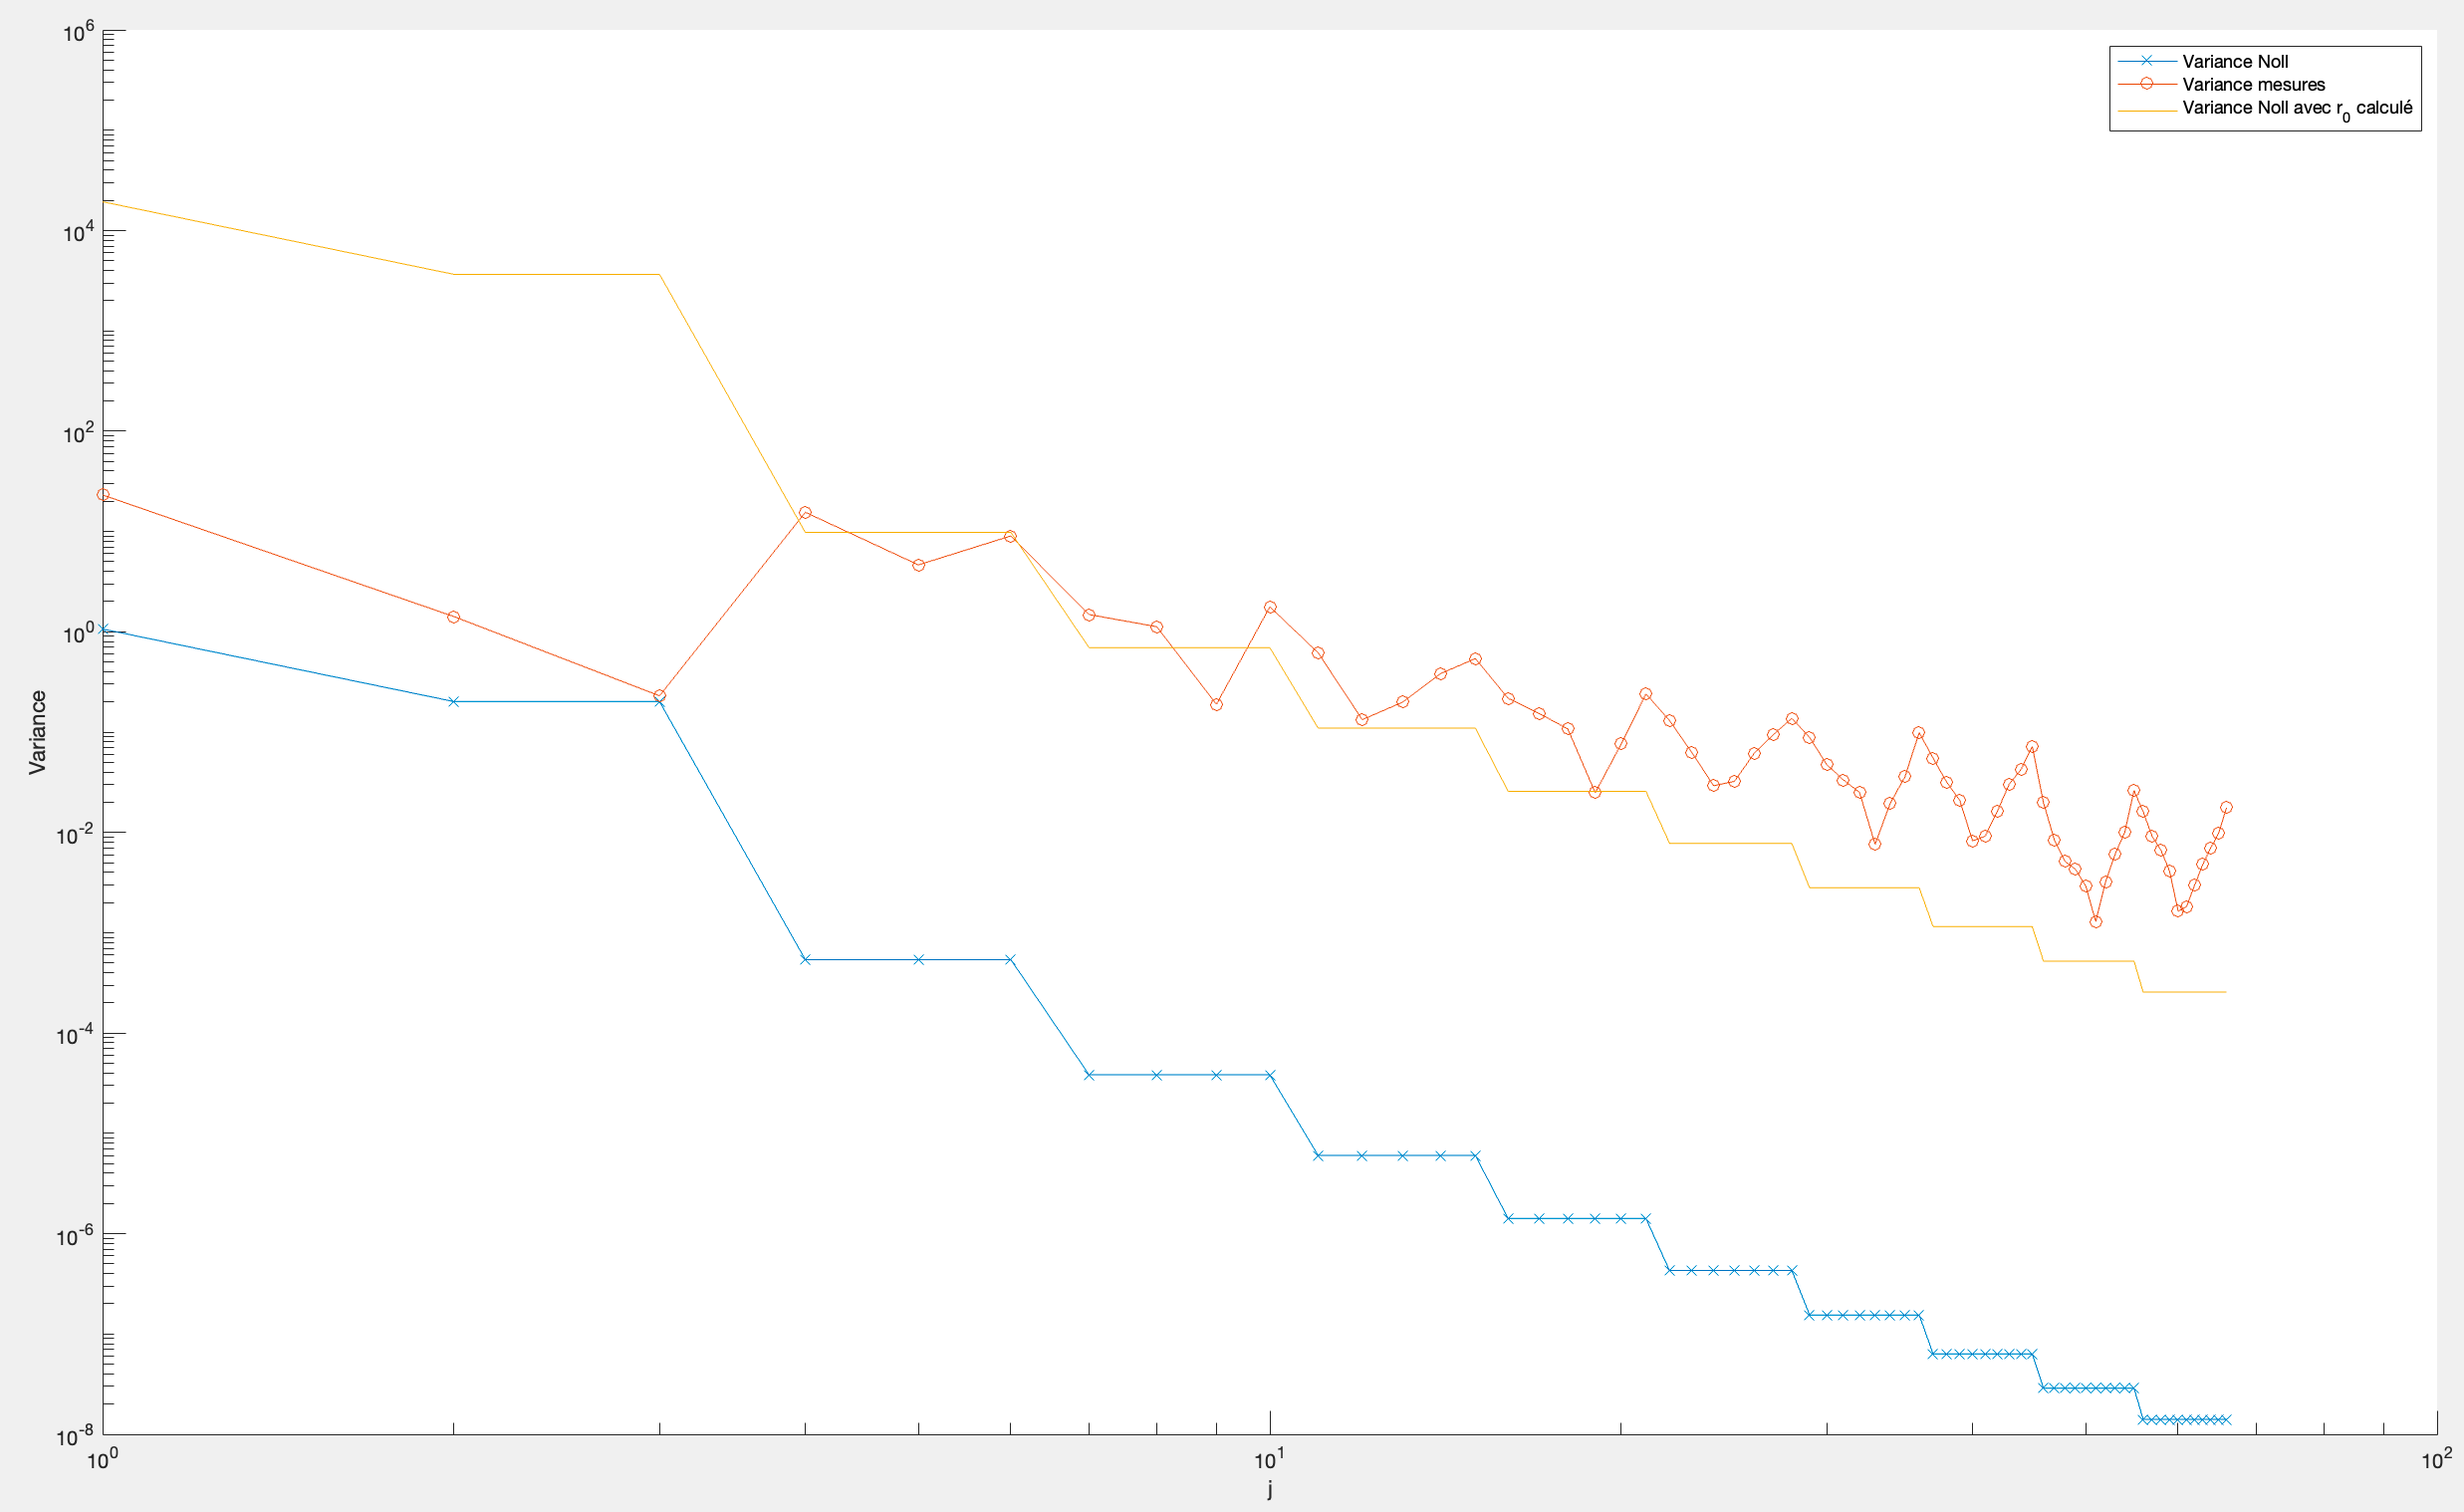
\includegraphics[width = \textwidth]{assets/figures/mesures/mesure_30_sec_1_plot.png}
    \caption{Graphique de la série consécutive 1}
\end{figure}
Le \textbf{$r_0$} calculé est égal à : \textbf{0.001949 cm}.

\subsection{Écran 60 secondes}
Ici une seule série de mesure a été réalisée selon les mêmes paramètres cités précédemment :
\begin{figure}[H]
    \centering
    
\includegraphics[width = 0.6\textwidth]{assets/figures/mesures/serie_mesures_60_sec.png}
    \caption{Série de mesures écran 60 secondes}
\end{figure}
\subsubsection{Mesure 60 secondes }
\begin{figure}[H]
    \centering
    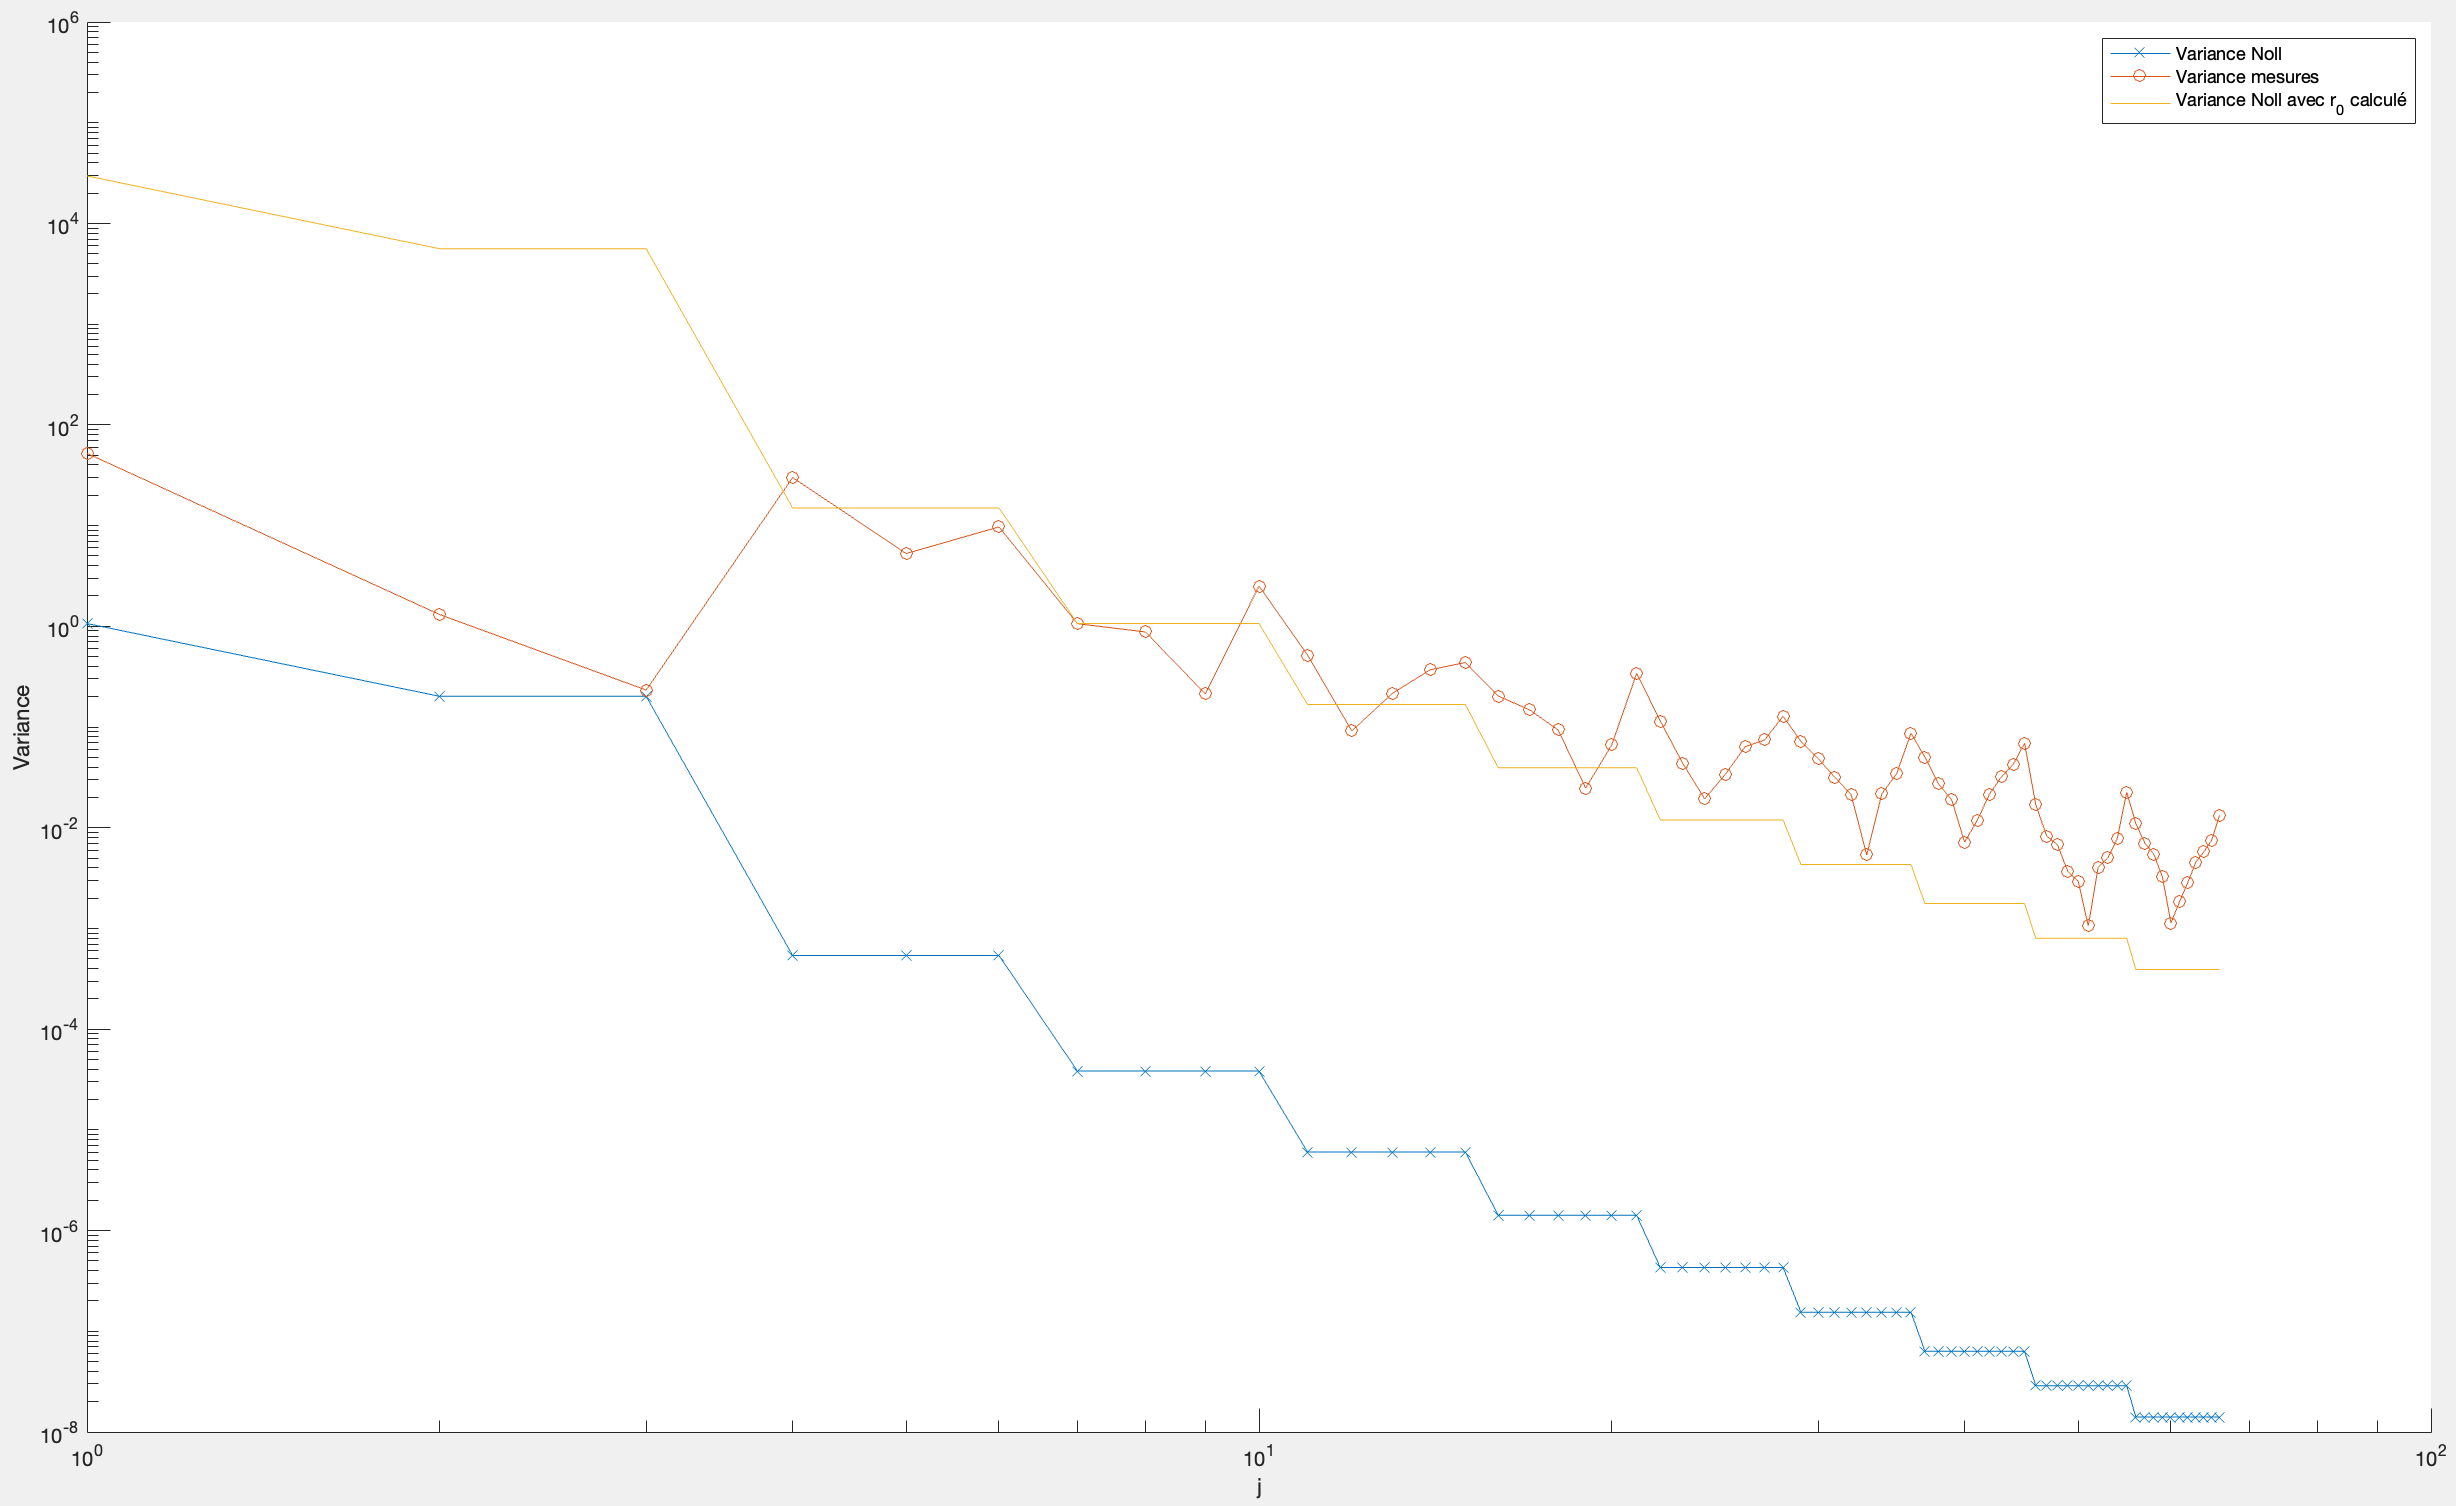
\includegraphics[width = \textwidth]{assets/figures/mesures/mesure_60_sec_1_plot.png}
    \caption{Graphique de la série de mesure}
\end{figure}
Le \textbf{$r_0$} calculé est égal à : \textbf{0.001949 cm}.
